\subsection{Plate with hole problem}\DIFaddbegin \label{subsec:plate_with_hole}
\DIFaddend Consider an infinite plate with a hole centered at the origin, as shown in Figure \ref{fg:plate_with_hole_model}, and at the infinity towards the $x$-direction subjected to a uniform traction $T=1000$. The geometric and material parameters for this problem are that the ratio of the hole $a=1$, Young's modulus $E=3\times 10^6$, and Poisson's ratio $\nu = 0.5-10^{-8}$. The analytical solution of this problem refers to the Michell solution \cite{timoshenko1969} as:
\begin{equation}\label{plate_with_hole_exact}
\left\{
\begin{aligned}
u_x(\rho,\theta)&=\frac{Ta}{8\mu}\left( \frac{\rho}{a}(k+1)\cos\theta - \frac{2a^3}{\rho^3}\cos3\theta + \frac{2a}{\rho}((1+k)\cos\theta + \cos3\theta) \right) \\
u_y(\rho,\theta)&=\frac{Ta}{8\mu}\left( \frac{\rho}{a}(k-3)\sin\theta - \frac{2a^3}{\rho^3}\sin3\theta + \frac{2a}{\rho}((1-k)\sin\theta + \sin3\theta) \right)
\end{aligned}
\right.
\end{equation}
in which $k = \frac{3-\nu}{1+\nu}$, $\mu = \frac{E}{2(1+\nu)}$. And the stress components are given by:
\begin{equation}
\left\{
\begin{aligned}
\sigma_{xx}&=T\left( 1 - \frac{a^2}{\rho^2}\left( \frac{3}{2}\cos2\theta + \cos4\theta \right) + \frac{3a^4}{2\rho^4}\cos4\theta \right) \\
\sigma_{yy}&=-T\left( \frac{a^2}{\rho^2}\left( \frac{1}{2}\cos2\theta - \cos4\theta \right) + \frac{3a^4}{2\rho^4}\cos4\theta \right) \\
\sigma_{xy}&=-T\left( \frac{a^2}{\rho^2}\left( \frac{1}{2}\sin2\theta + \sin4\theta \right) - \frac{3a^4}{2\rho^4}\sin4\theta \right) \\
\end{aligned}
\right.
\end{equation}

\begin{figure}[h!]
\centering
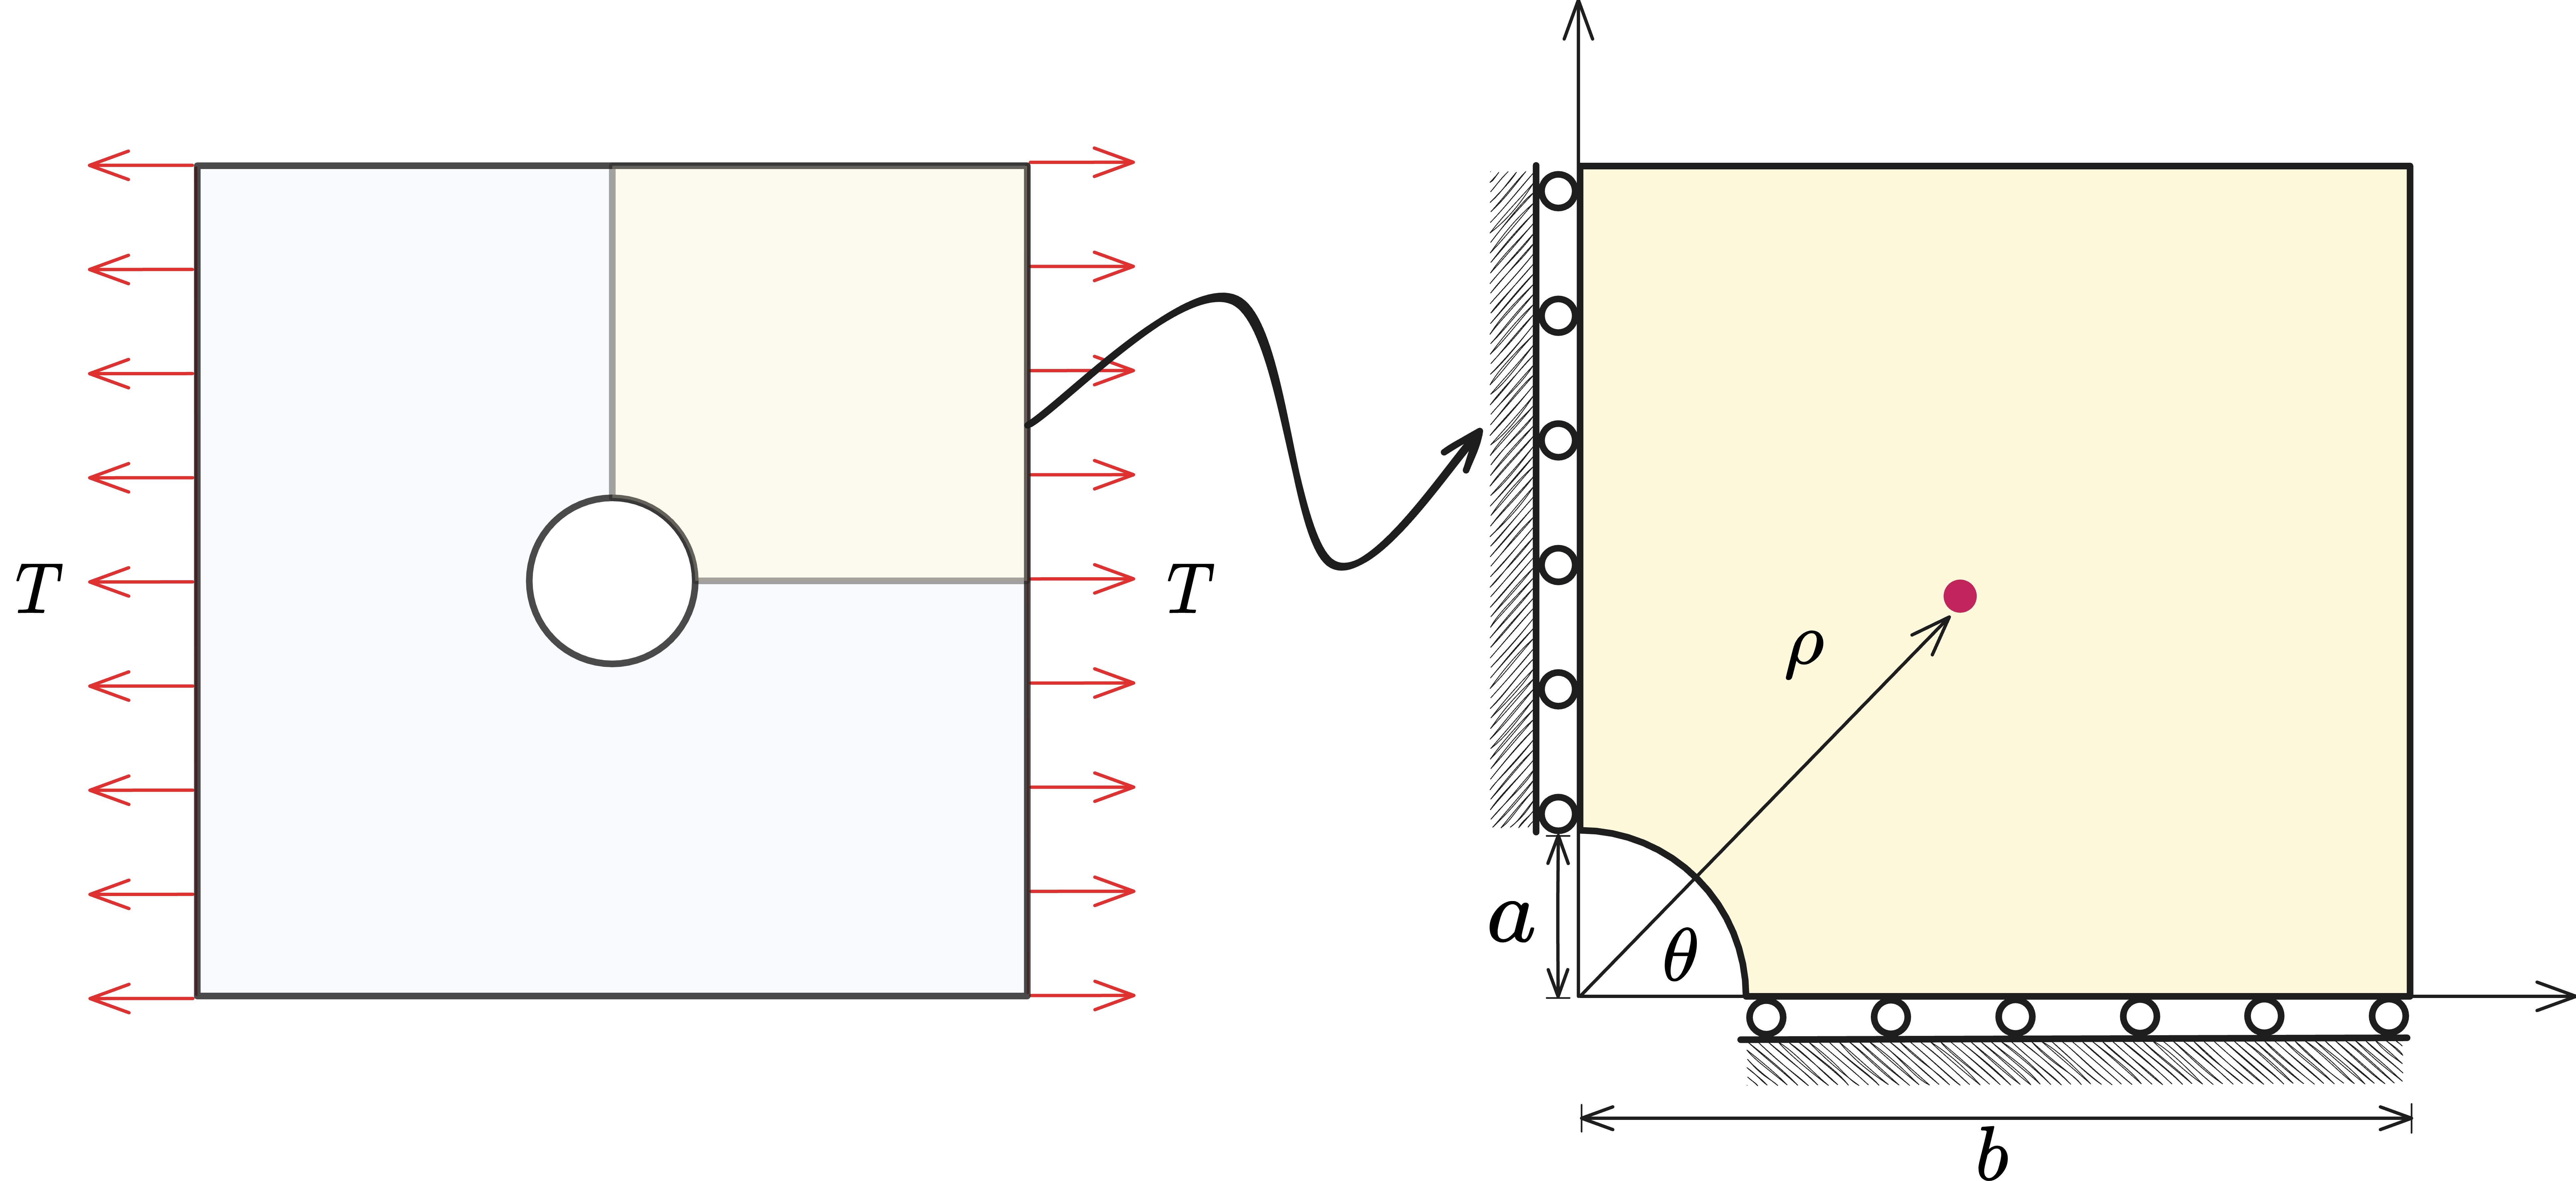
\includegraphics[width=\textwidth]{png/plate_with_hole_model.png}
\caption{Illustration of plate with hole problem}\label{fg:plate_with_hole_model}
\end{figure}

According to the symmetry property of this problem, only a quarter model with length $b=5$ is considered as shown in Figure \ref{fg:plate_with_hole_model}. The displacement is discretized by 3-node \DIFaddbegin \DIFadd{, }\DIFaddend 6-node triangular elements ,  \DIFaddbegin \DIFadd{4-node and 8-node quadrilateral elements}\DIFaddend . The corresponding linear and quadratic meshfree formulations are employed for pressure discretization, and the characterized support sizes are chosen as 1.5 and 2.5, respectively.
 \DIFaddbegin \DIFadd{Figures \ref{fg:plate_with_hole_ns}, \ref{fg:plate_with_hole_quad_ns} study }\DIFaddend the relationship between strain, pressure errors, and $n_p$ using the nodal distributions uniformly related to displacement nodes.
Unlike the quadrilateral element case in Section \ref{sec:cantilever},  \DIFaddbegin \DIFadd{both displacement and pressure errors in this problem increase as $n_p$ reduces to a small value.
}\DIFaddend Tri3--RK exhibits less sensitivity in strain error than Tri6--RK \DIFaddbegin \DIFadd{.
This is because, as shown in Eqs. \eqref{u_estimator} and \eqref{kerp_estimator}, the displacement approximation error for the space of $\ker \mathcal P_h$ does not increase as immediately when $\frac{C_b}{\beta}$ in Eq. \eqref{kerp_estimator} is not too much larger than 1.
However, its error increases as }\DIFaddend $n_p$ goes up.
Both  \DIFaddbegin \DIFadd{FE--RK }\DIFaddend with constraint ratios under the optimal range perform acceptably. 

\begin{figure}[!htp]
\centering
\begin{tabular}{c@{\hspace{0pt}}c}
$\Vert \boldsymbol{u} - \boldsymbol{u}_h \Vert_V$ & $\Vert p - p_h \Vert_Q$ \\
\raisebox{-0.7\height}{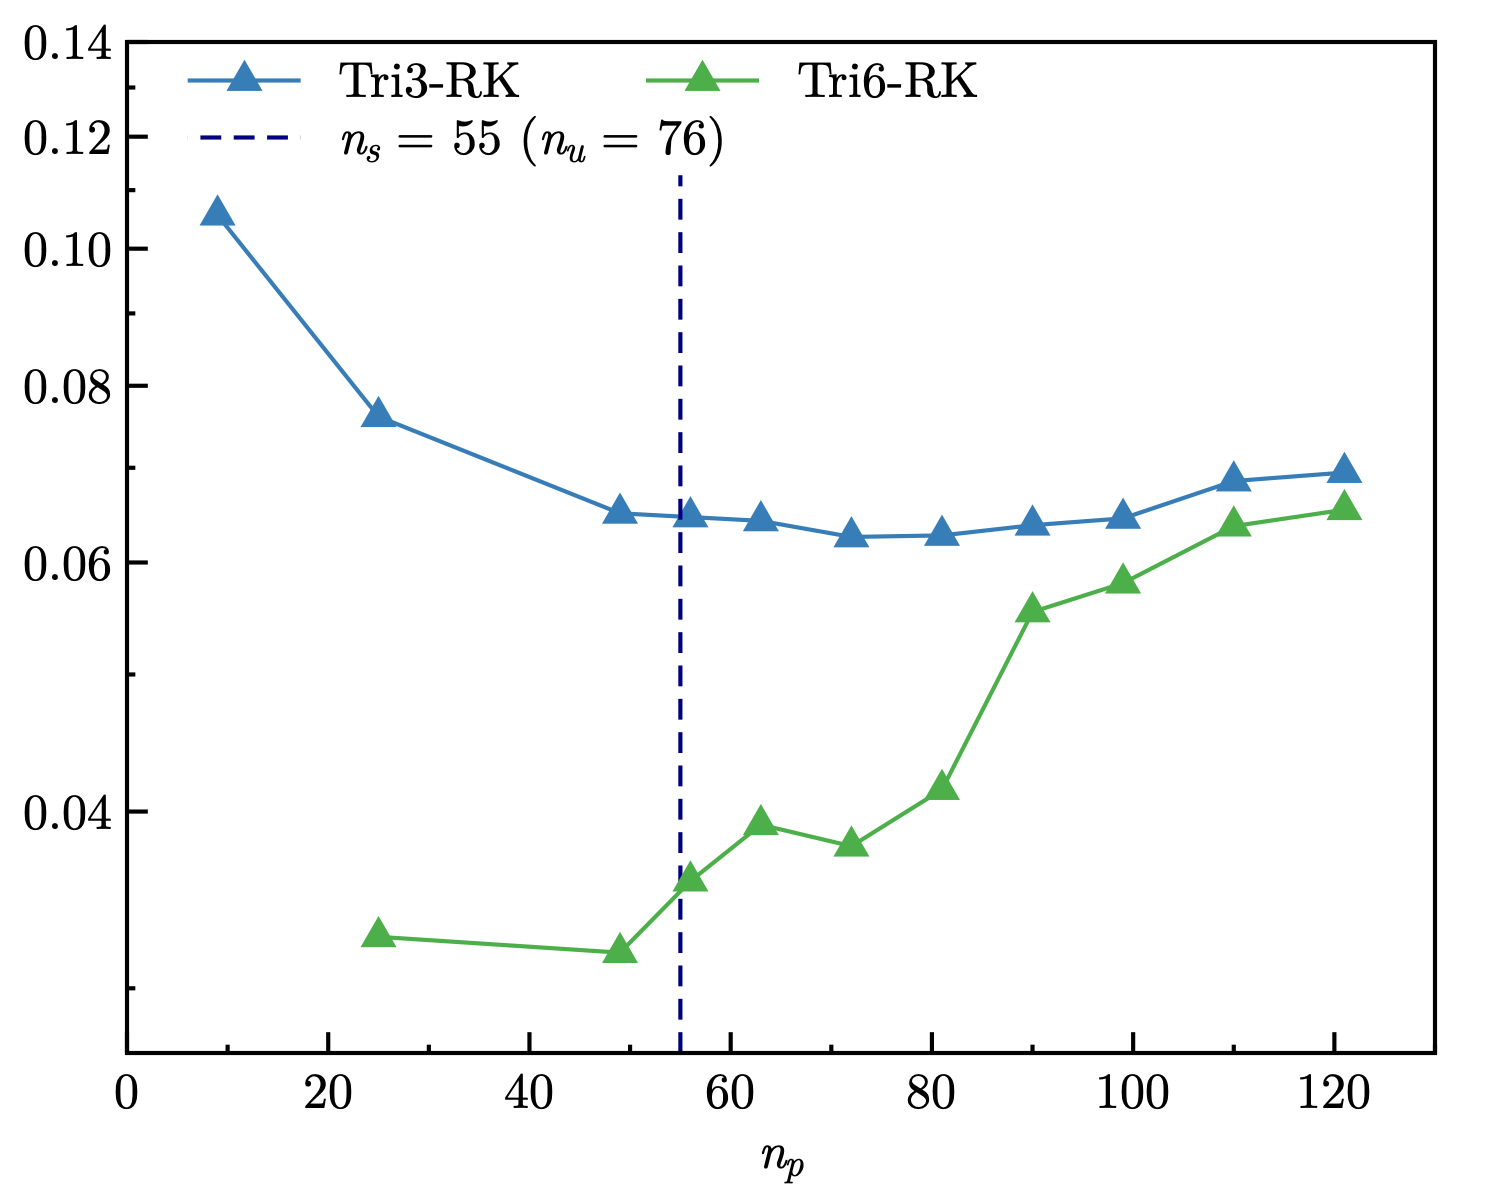
\includegraphics[width=0.48\textwidth]{png/plate_Hdev_4.png}}
& \raisebox{-0.7\height}{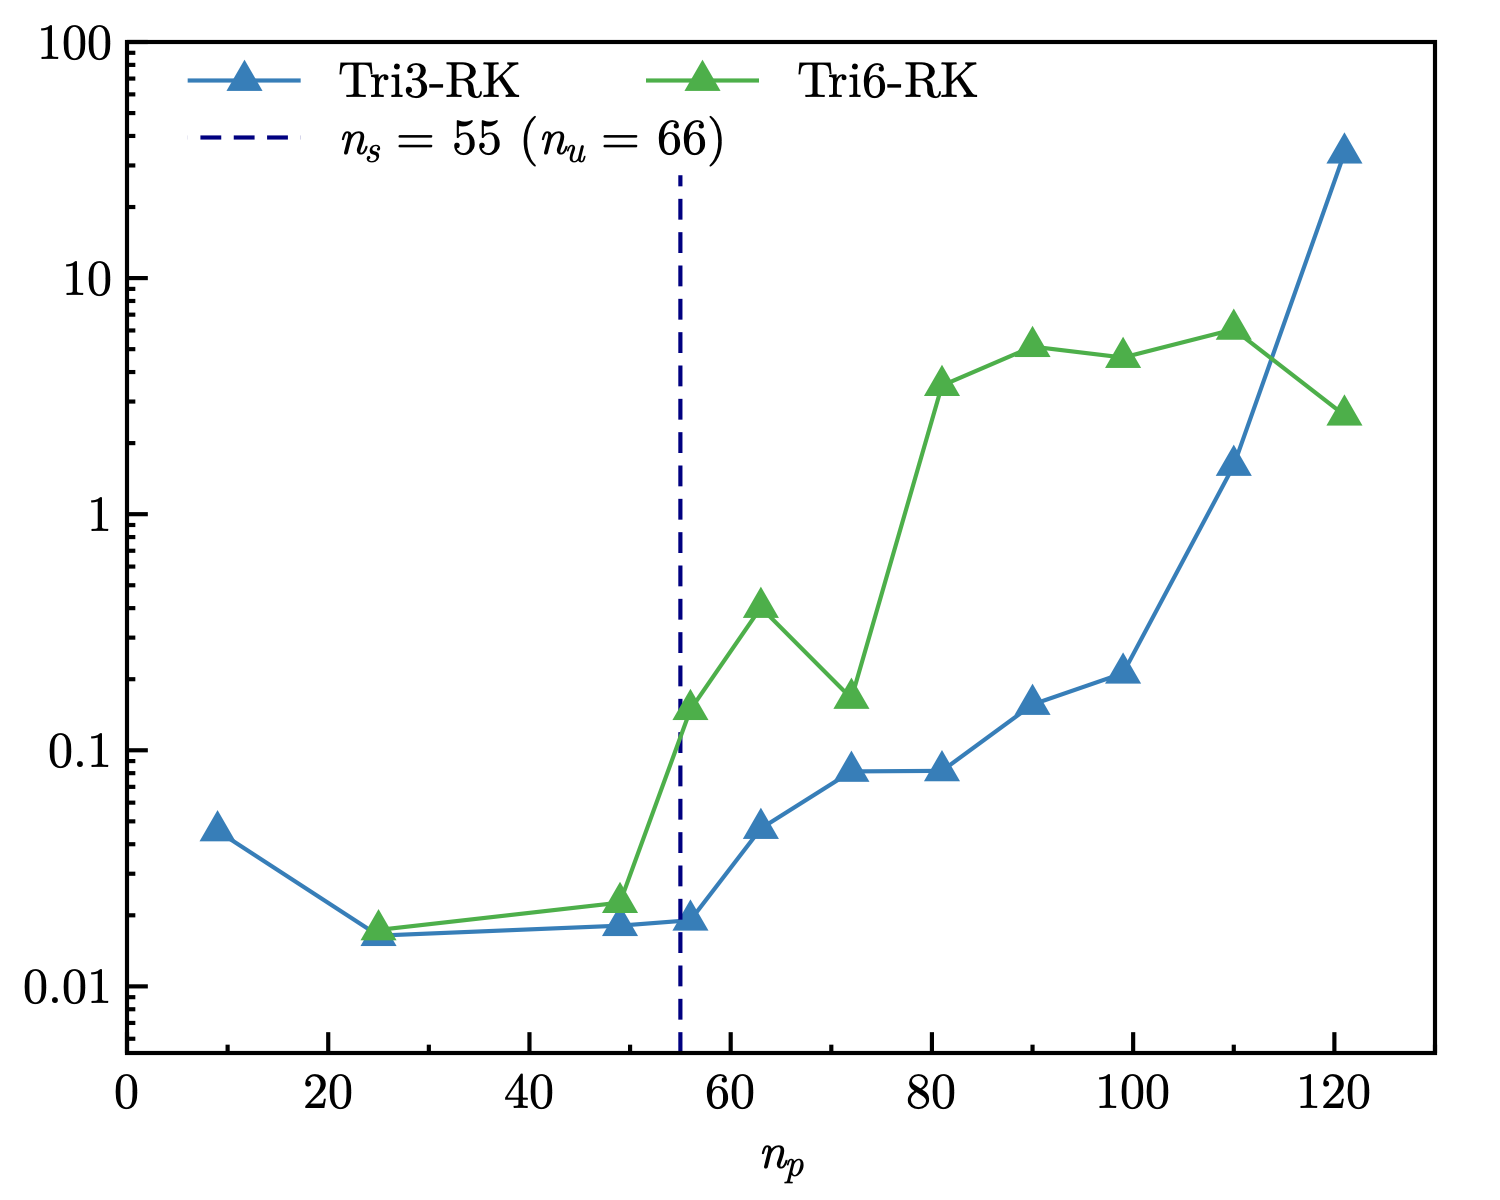
\includegraphics[width=0.48\textwidth]{png/plate_L2_p_4.png}} \\
\raisebox{-0.7\height}{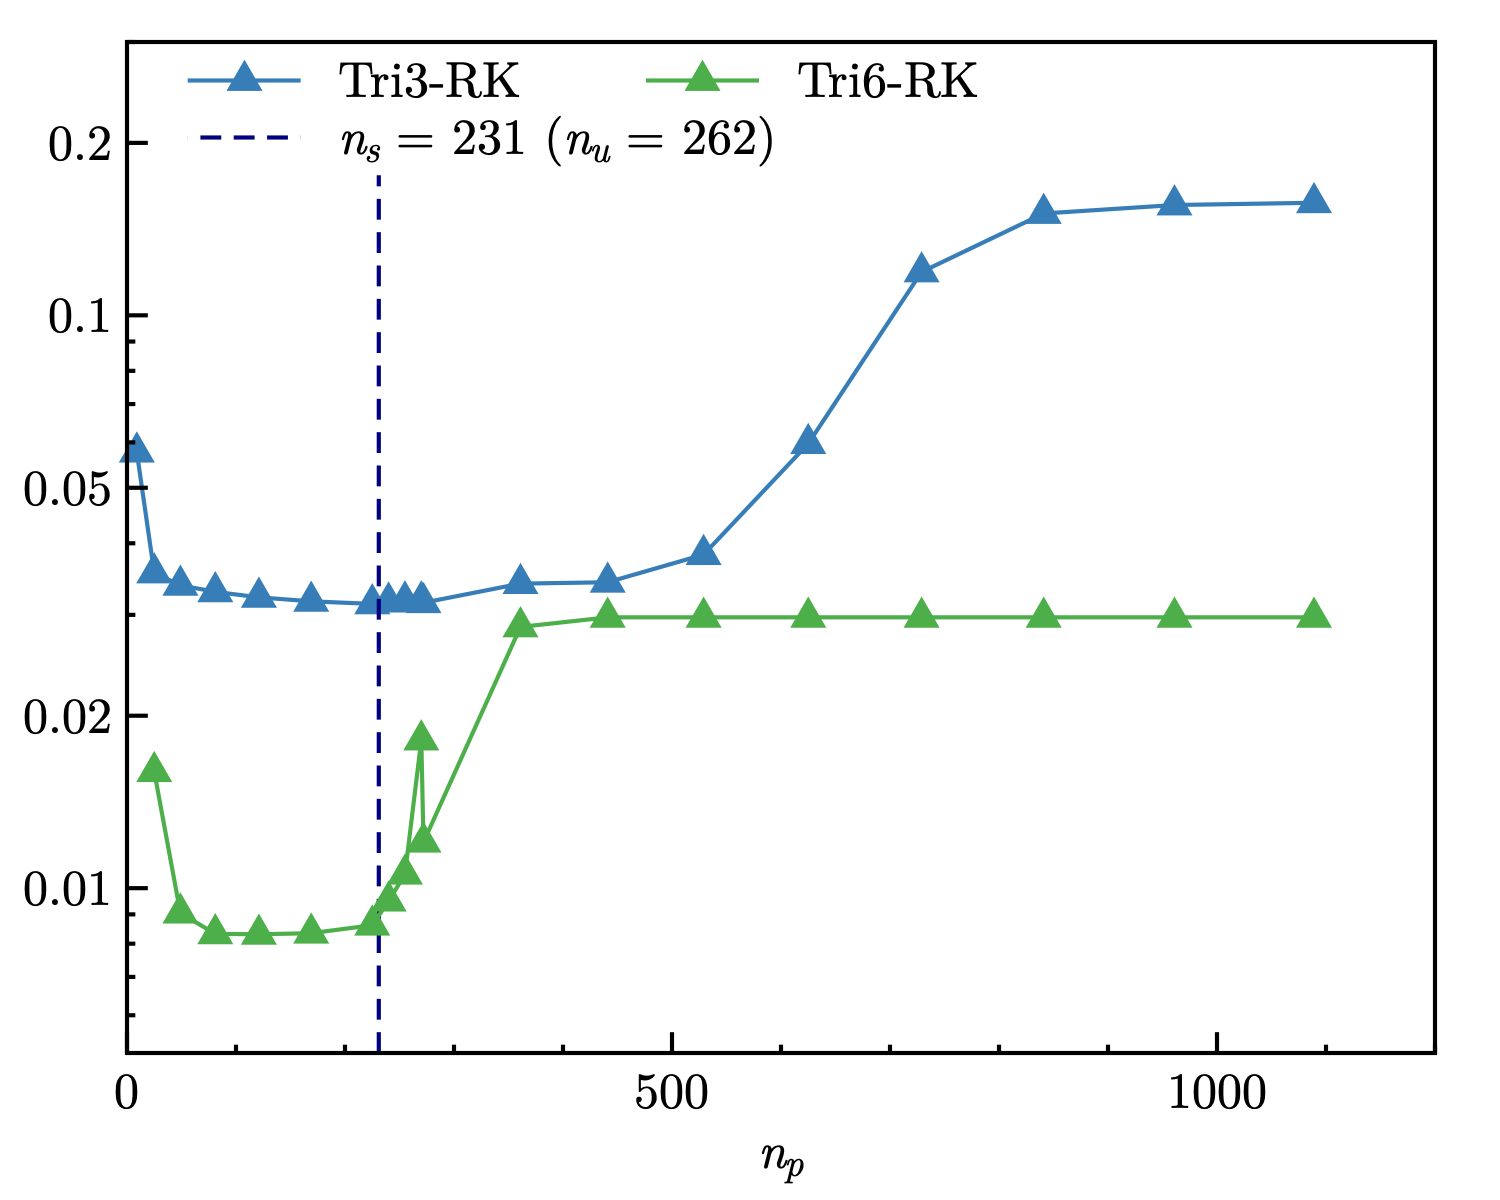
\includegraphics[width=0.48\textwidth]{png/plate_Hdev_8.png}}
& \raisebox{-0.7\height}{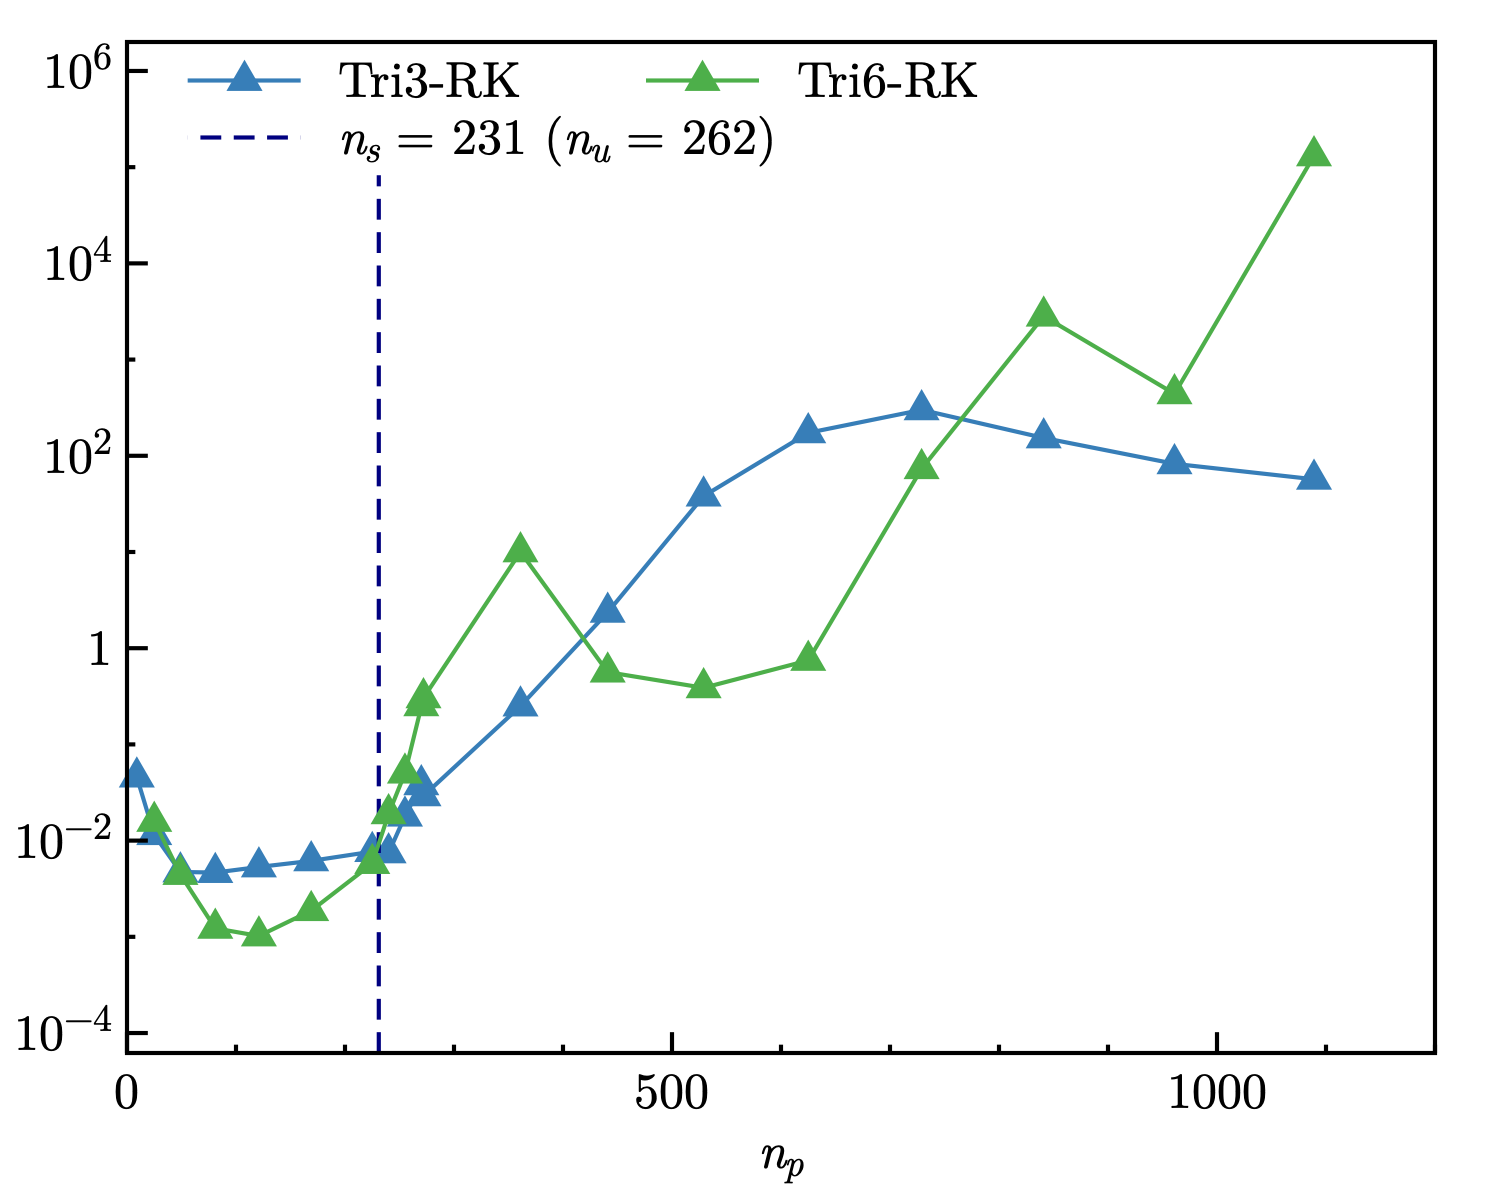
\includegraphics[width=0.48\textwidth]{png/plate_L2_p_8.png}} \\
\raisebox{-0.7\height}{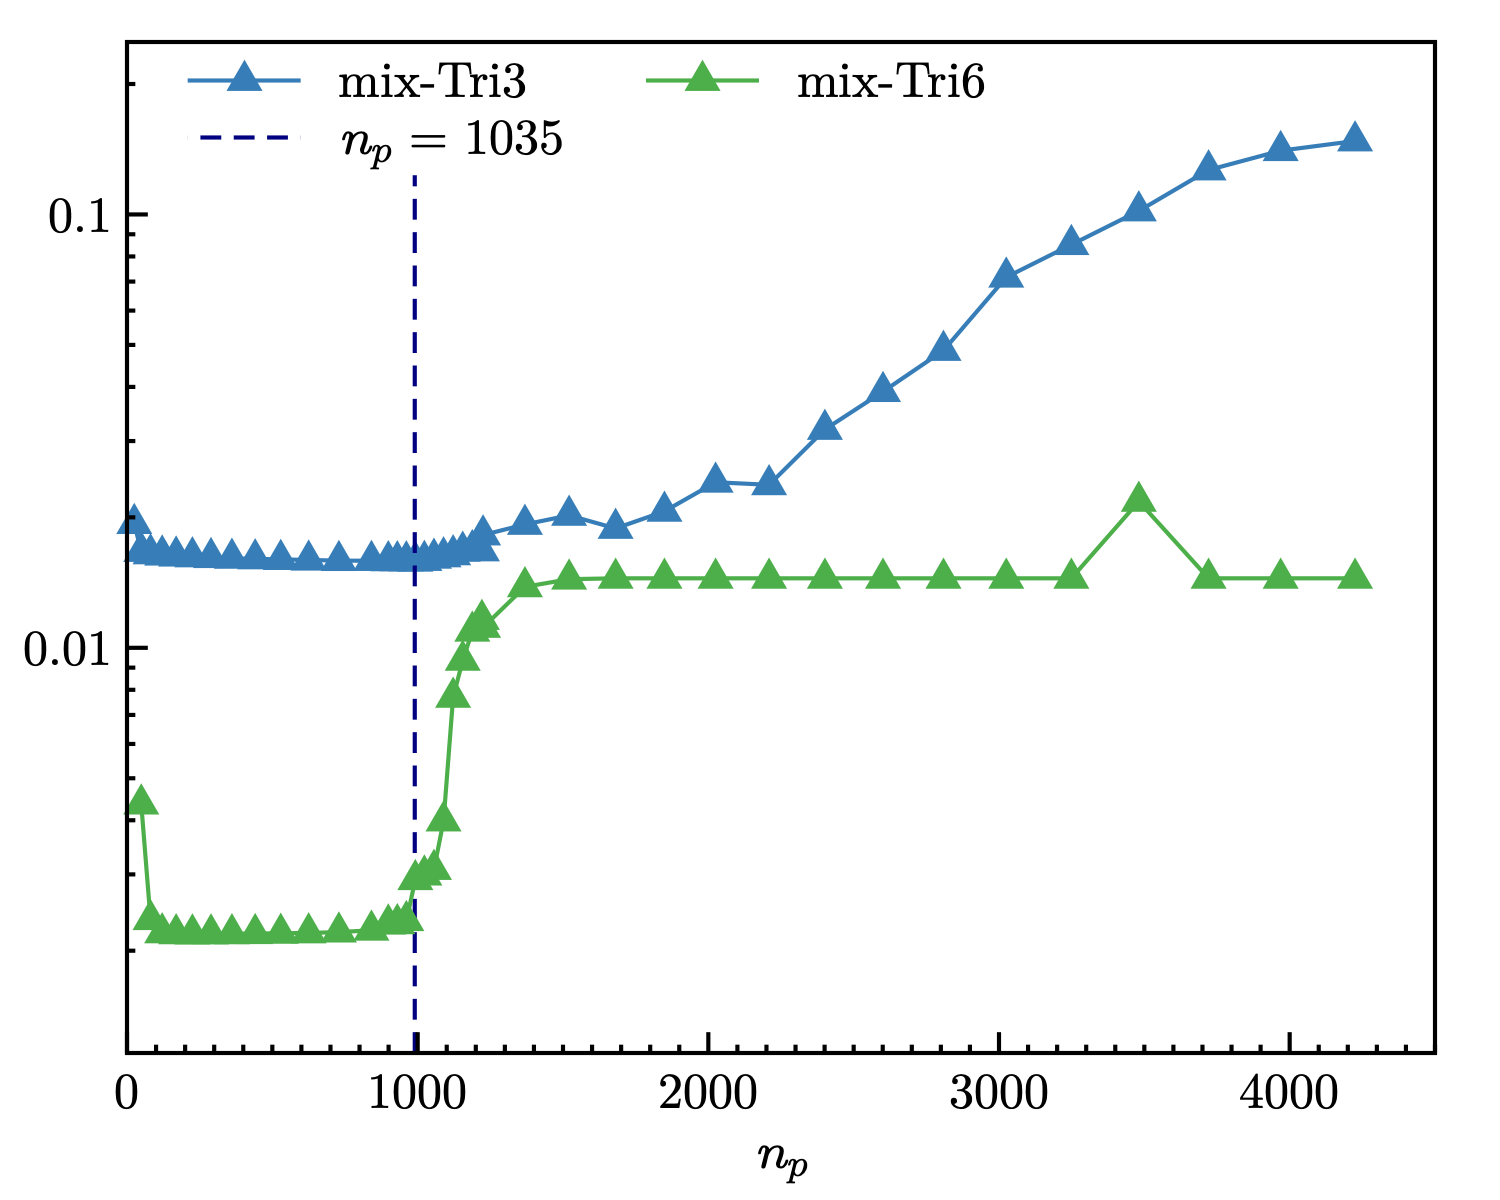
\includegraphics[width=0.48\textwidth]{png/plate_Hdev_16.png}}
& \raisebox{-0.7\height}{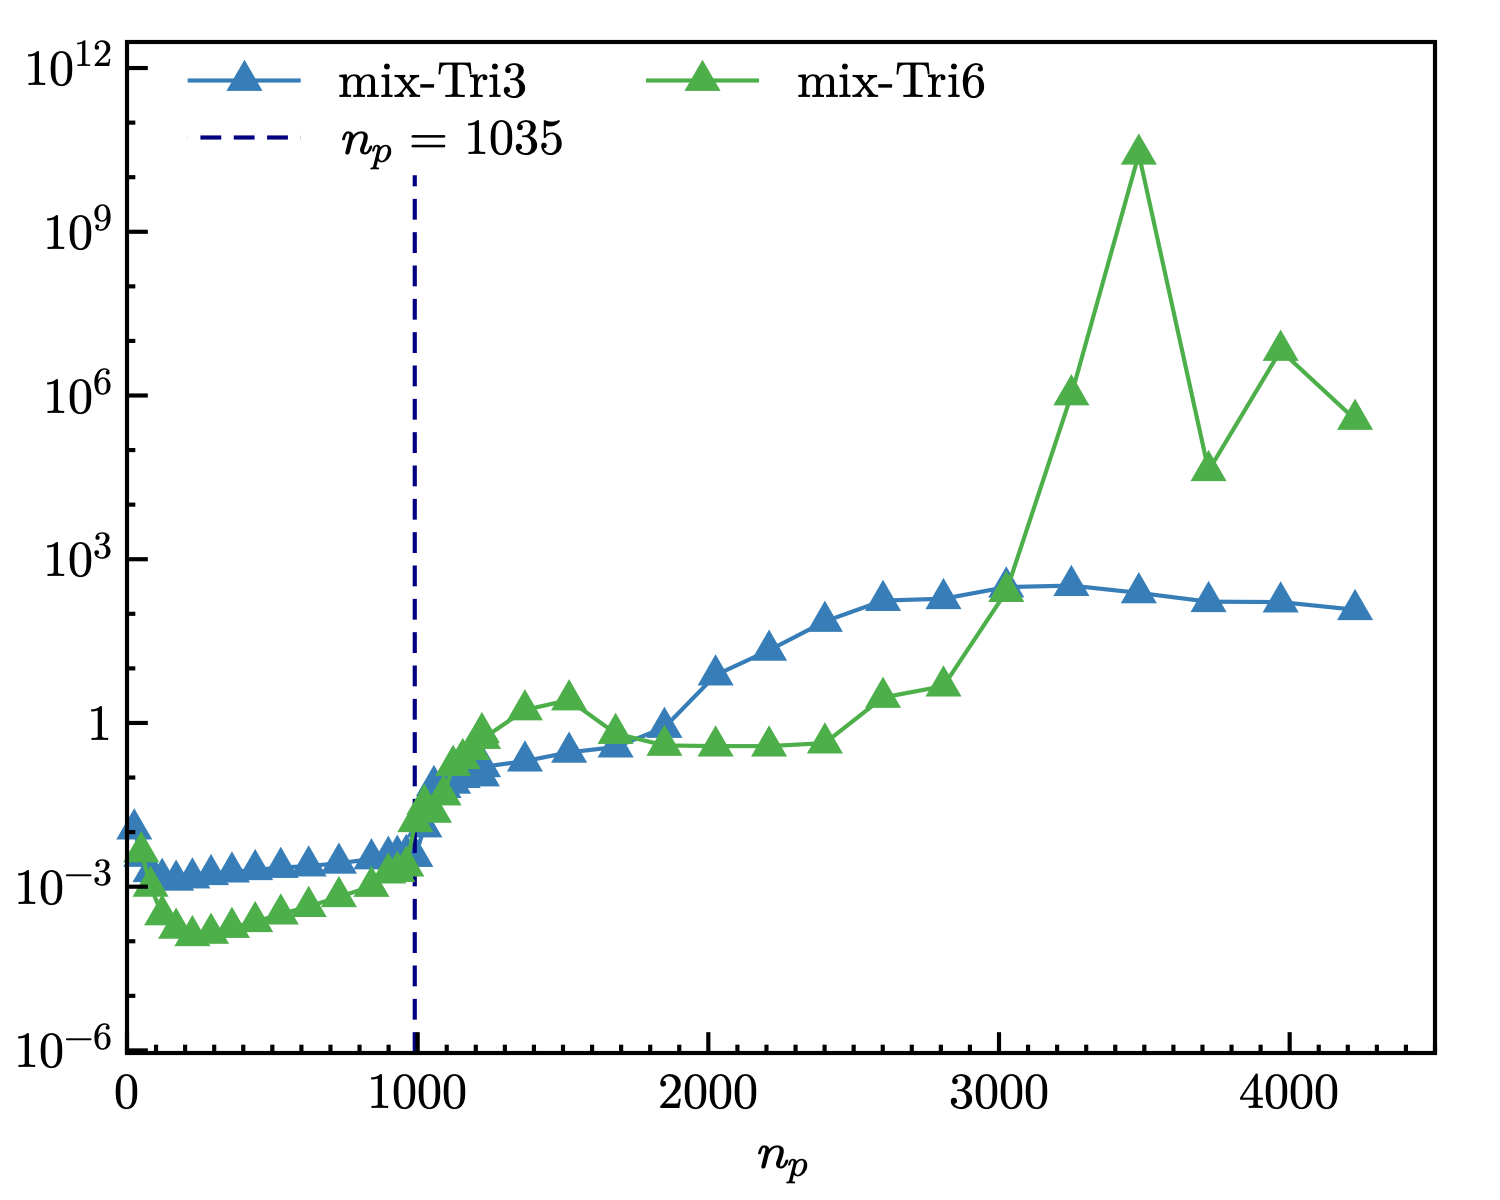
\includegraphics[width=0.48\textwidth]{png/plate_L2_p_16.png}} \\
\raisebox{-0.7\height}{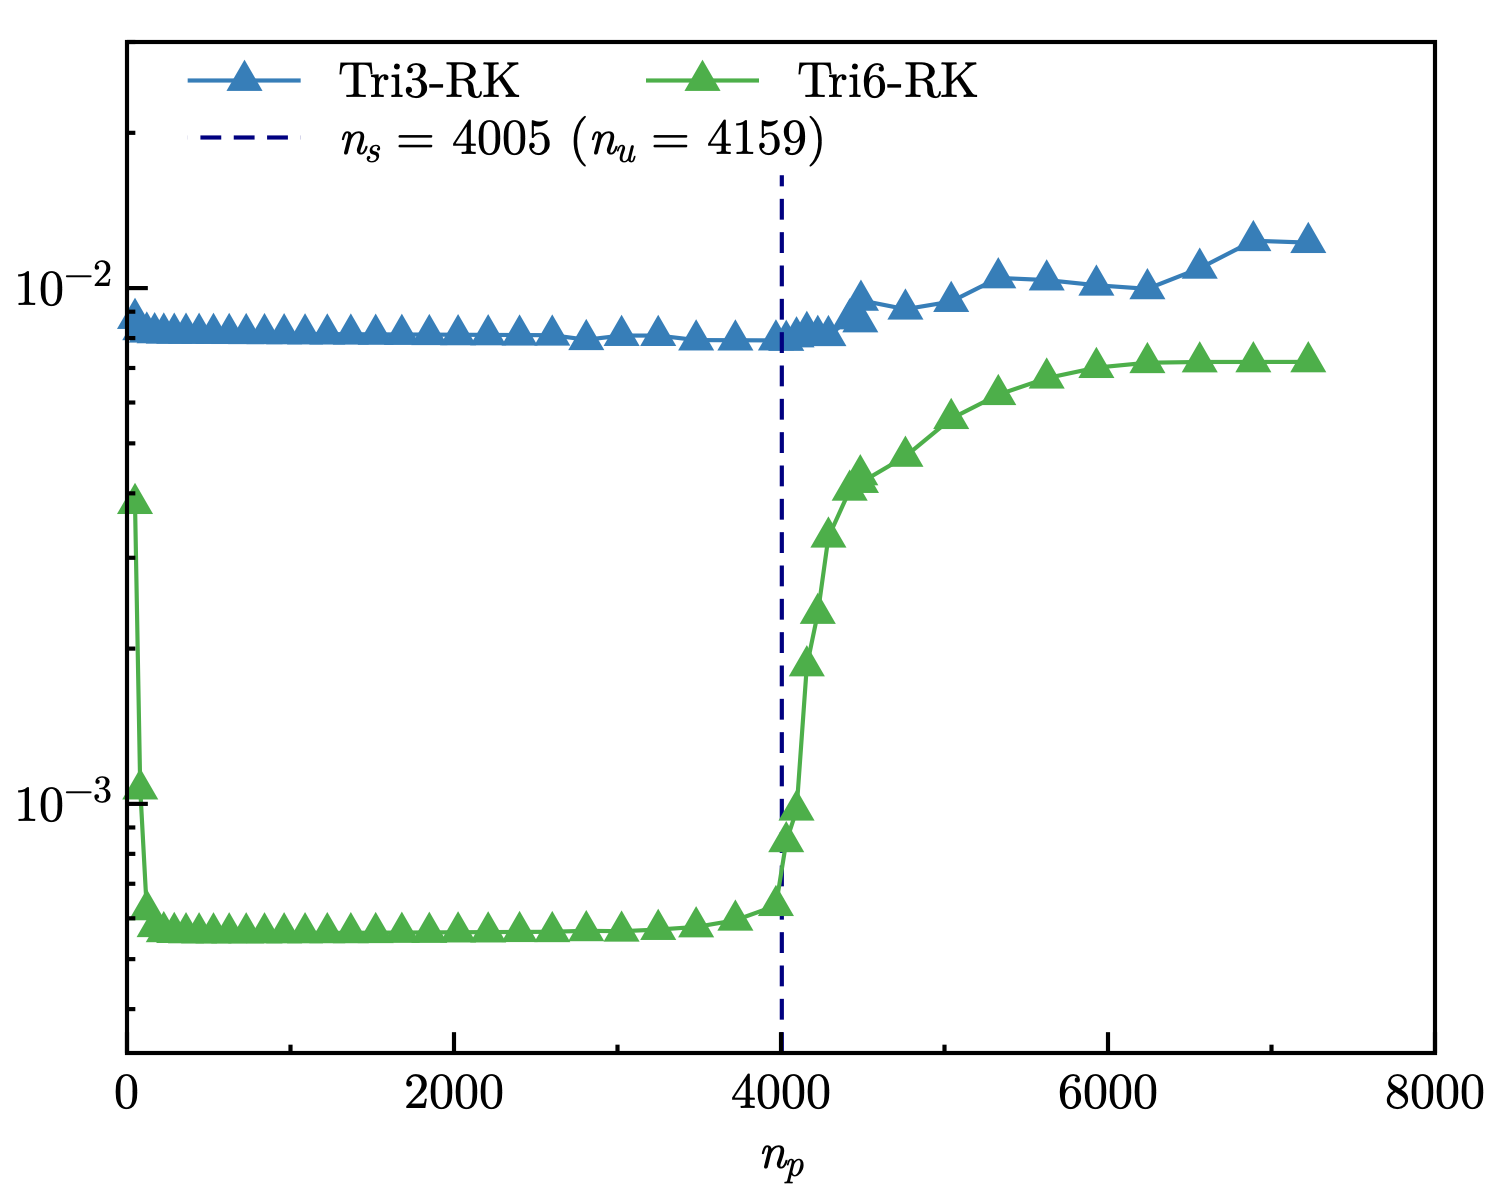
\includegraphics[width=0.48\textwidth]{png/plate_Hdev_32.png}}
& \raisebox{-0.7\height}{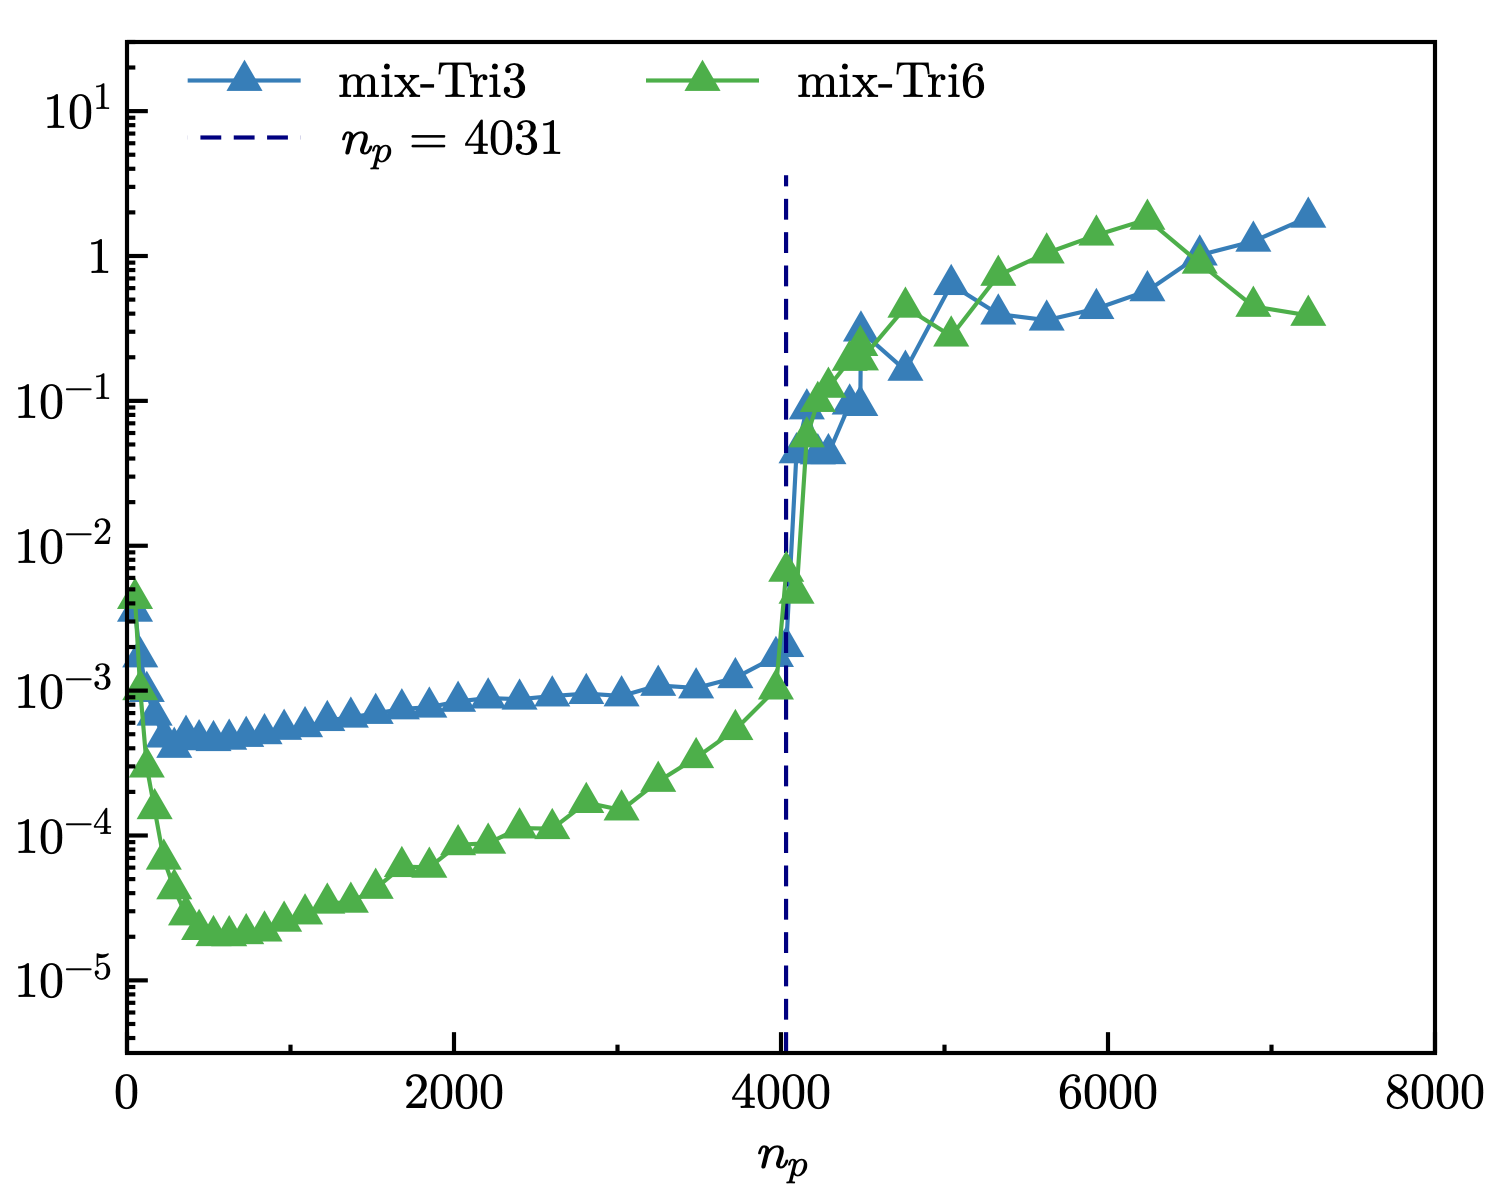
\includegraphics[width=0.48\textwidth]{png/plate_L2_p_32.png}} \\
\end{tabular}
\caption{Strain and pressure errors vs. $n_p$ for plate with hole problem \DIFaddFL{with triangular elements}}\label{fg:plate_with_hole_ns}
\end{figure}

\DIFaddbegin 
\begin{figure}[!htp]
\centering
\begin{tabular}{c@{\hspace{0pt}}c}
\DIFaddFL{$\Vert \boldsymbol{u} - \boldsymbol{u}_h \Vert_V$ }& \DIFaddFL{$\Vert p - p_h \Vert_Q$ }\\
\DIFaddFL{\raisebox{-0.7\height}{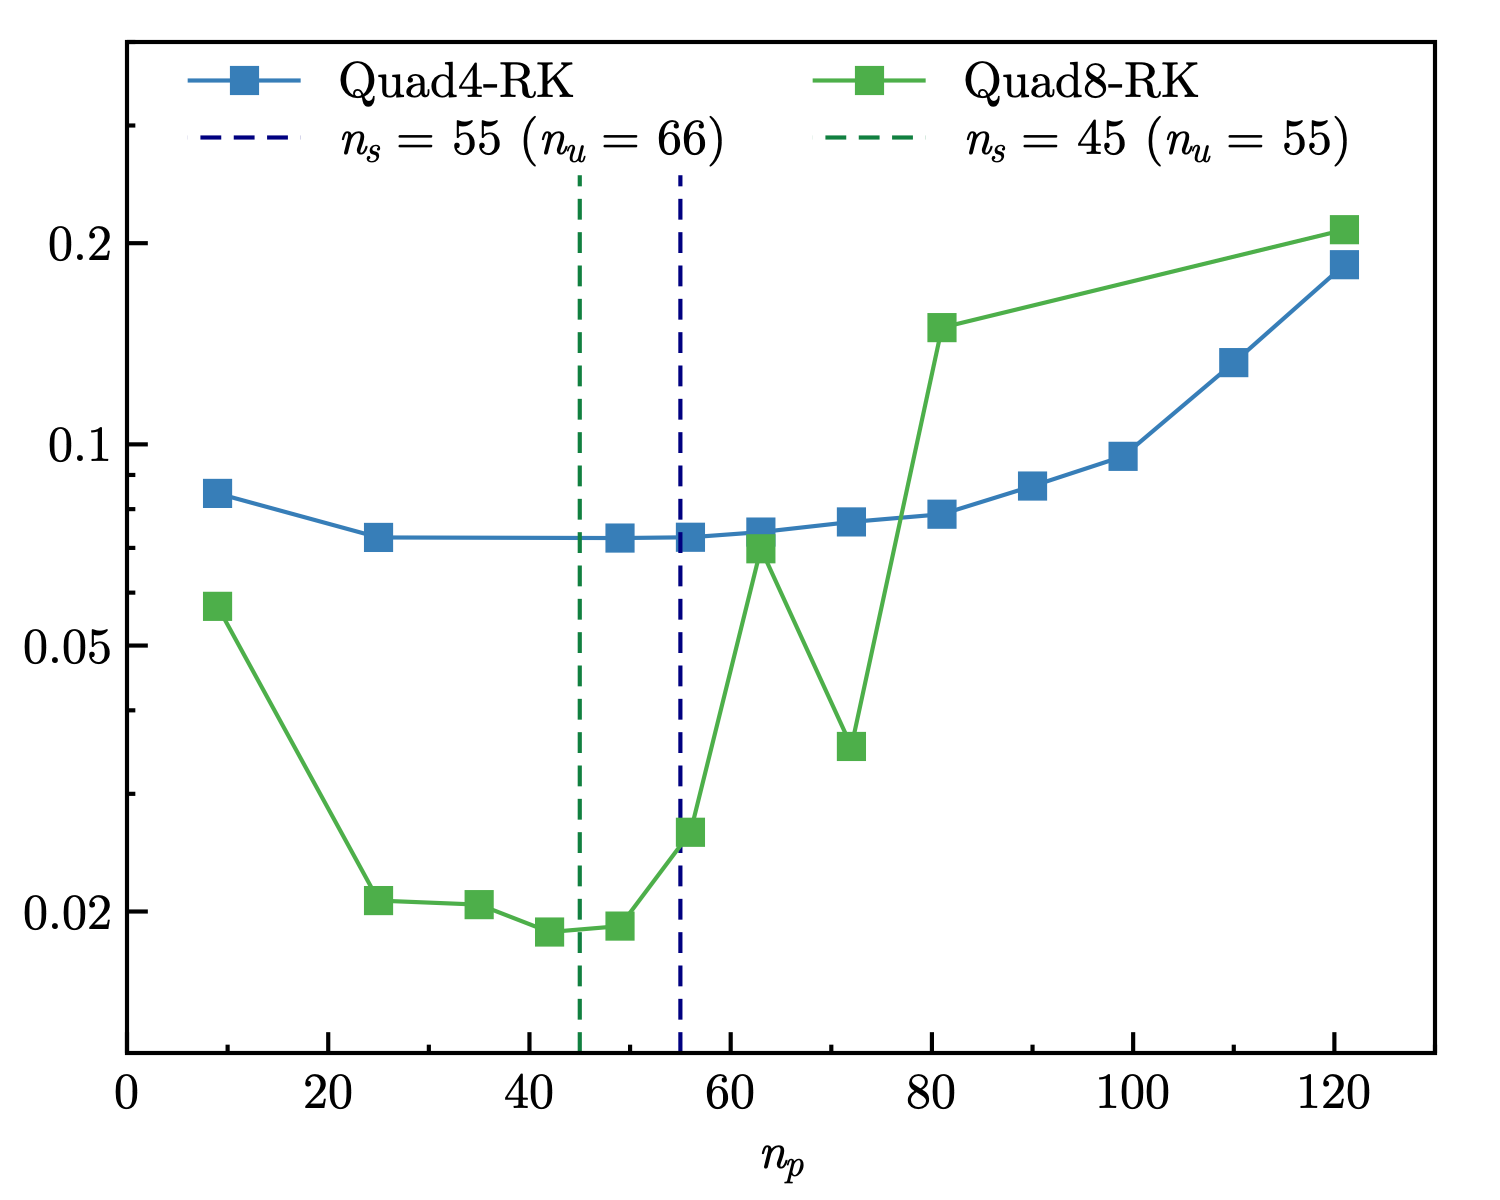
\includegraphics[width=0.48\textwidth]{png/plate_with_hole_quad_Hdev_4.png}}
}& \DIFaddFL{\raisebox{-0.7\height}{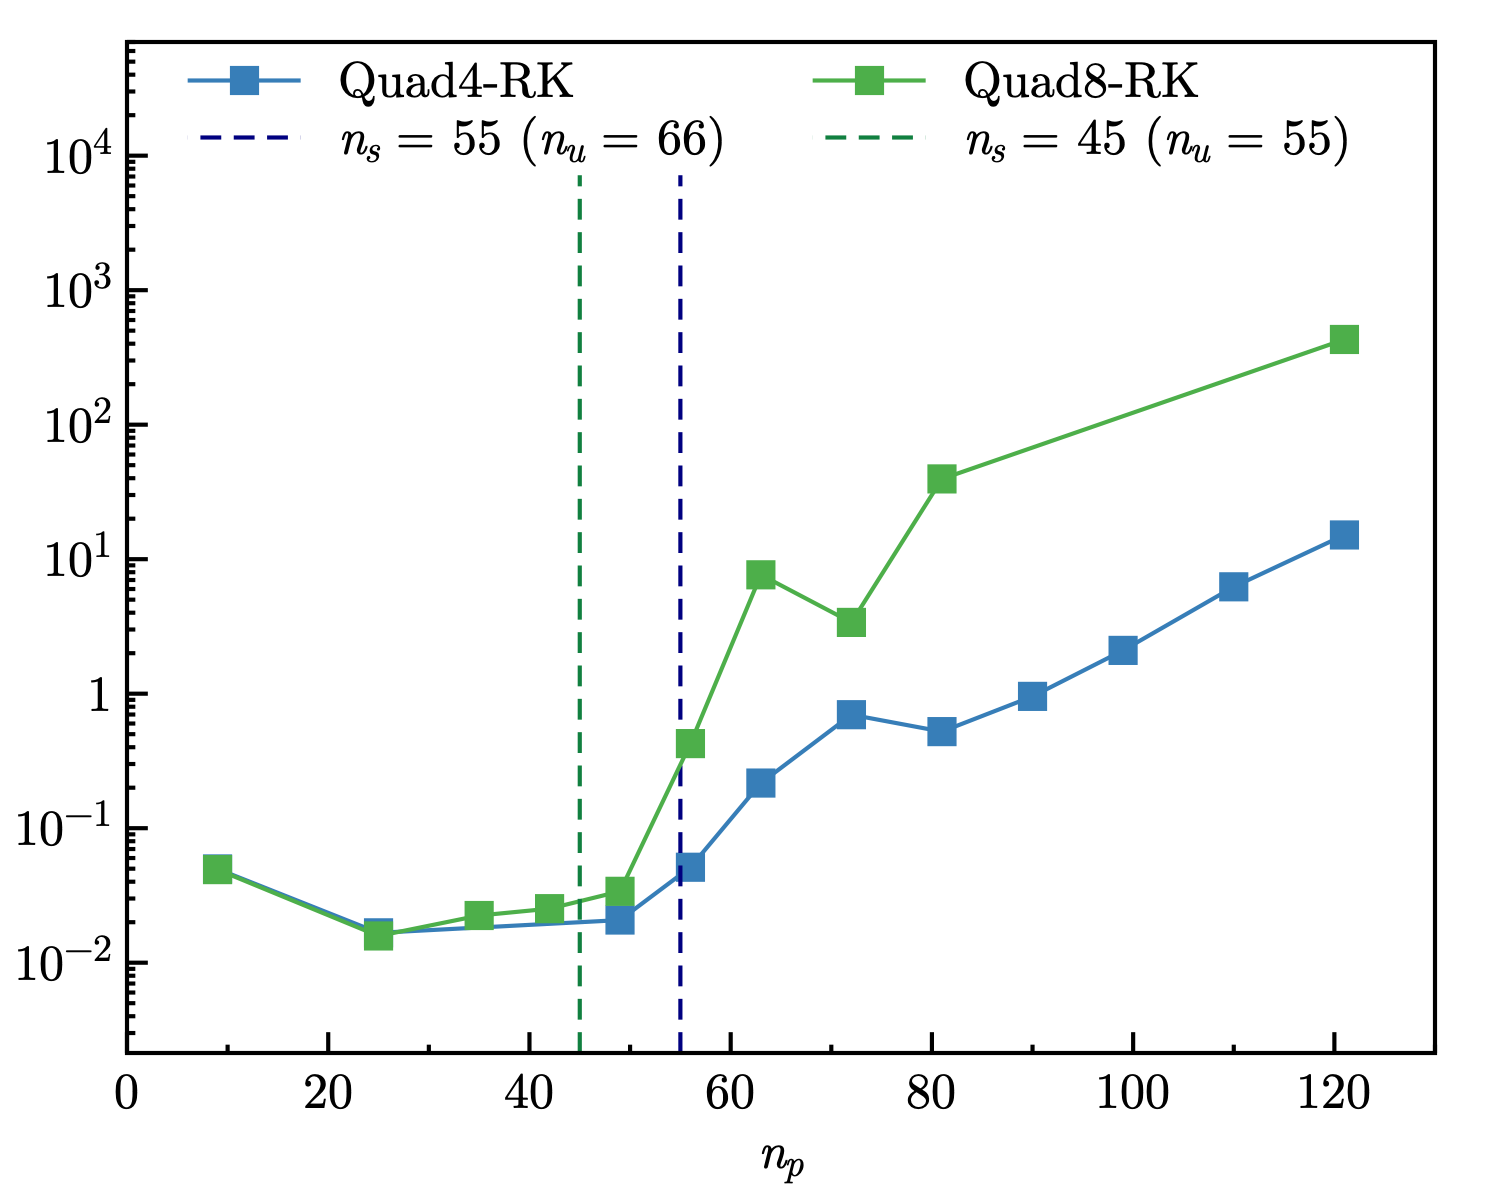
\includegraphics[width=0.48\textwidth]{png/plate_with_hole_quad_L2_p_4.png}} }\\
\DIFaddFL{\raisebox{-0.7\height}{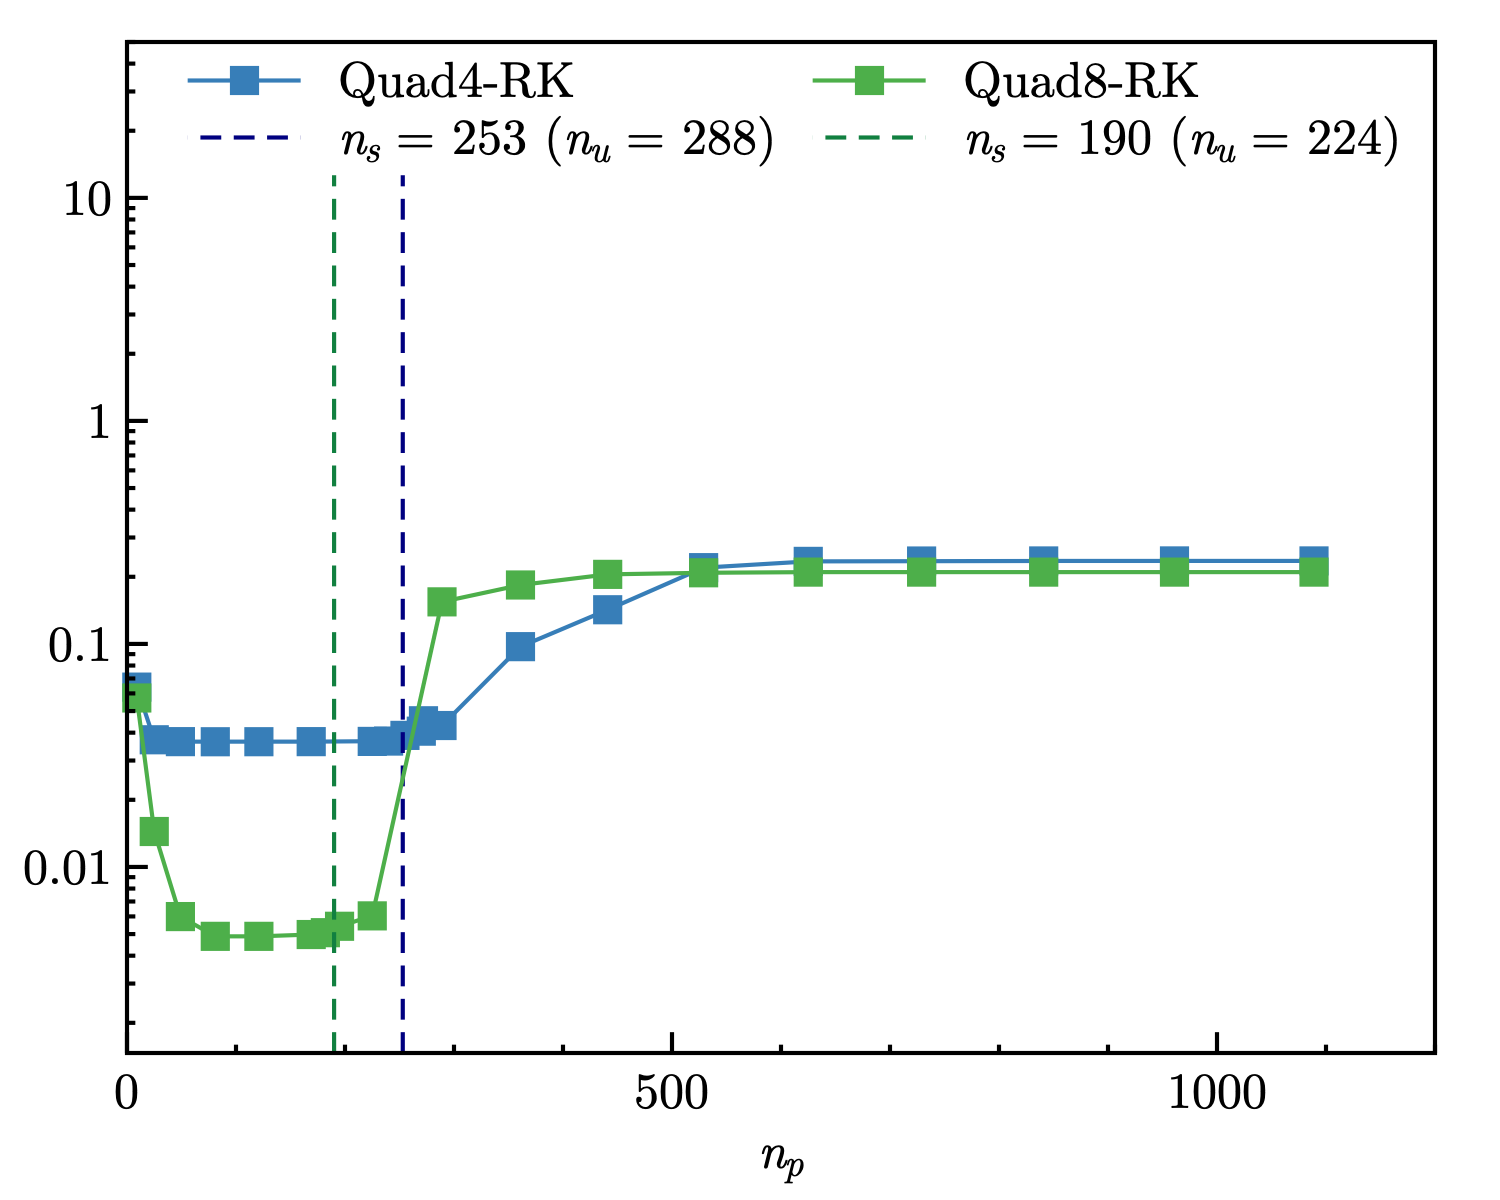
\includegraphics[width=0.48\textwidth]{png/plate_with_hole_quad_Hdev_8.png}}
}& \DIFaddFL{\raisebox{-0.7\height}{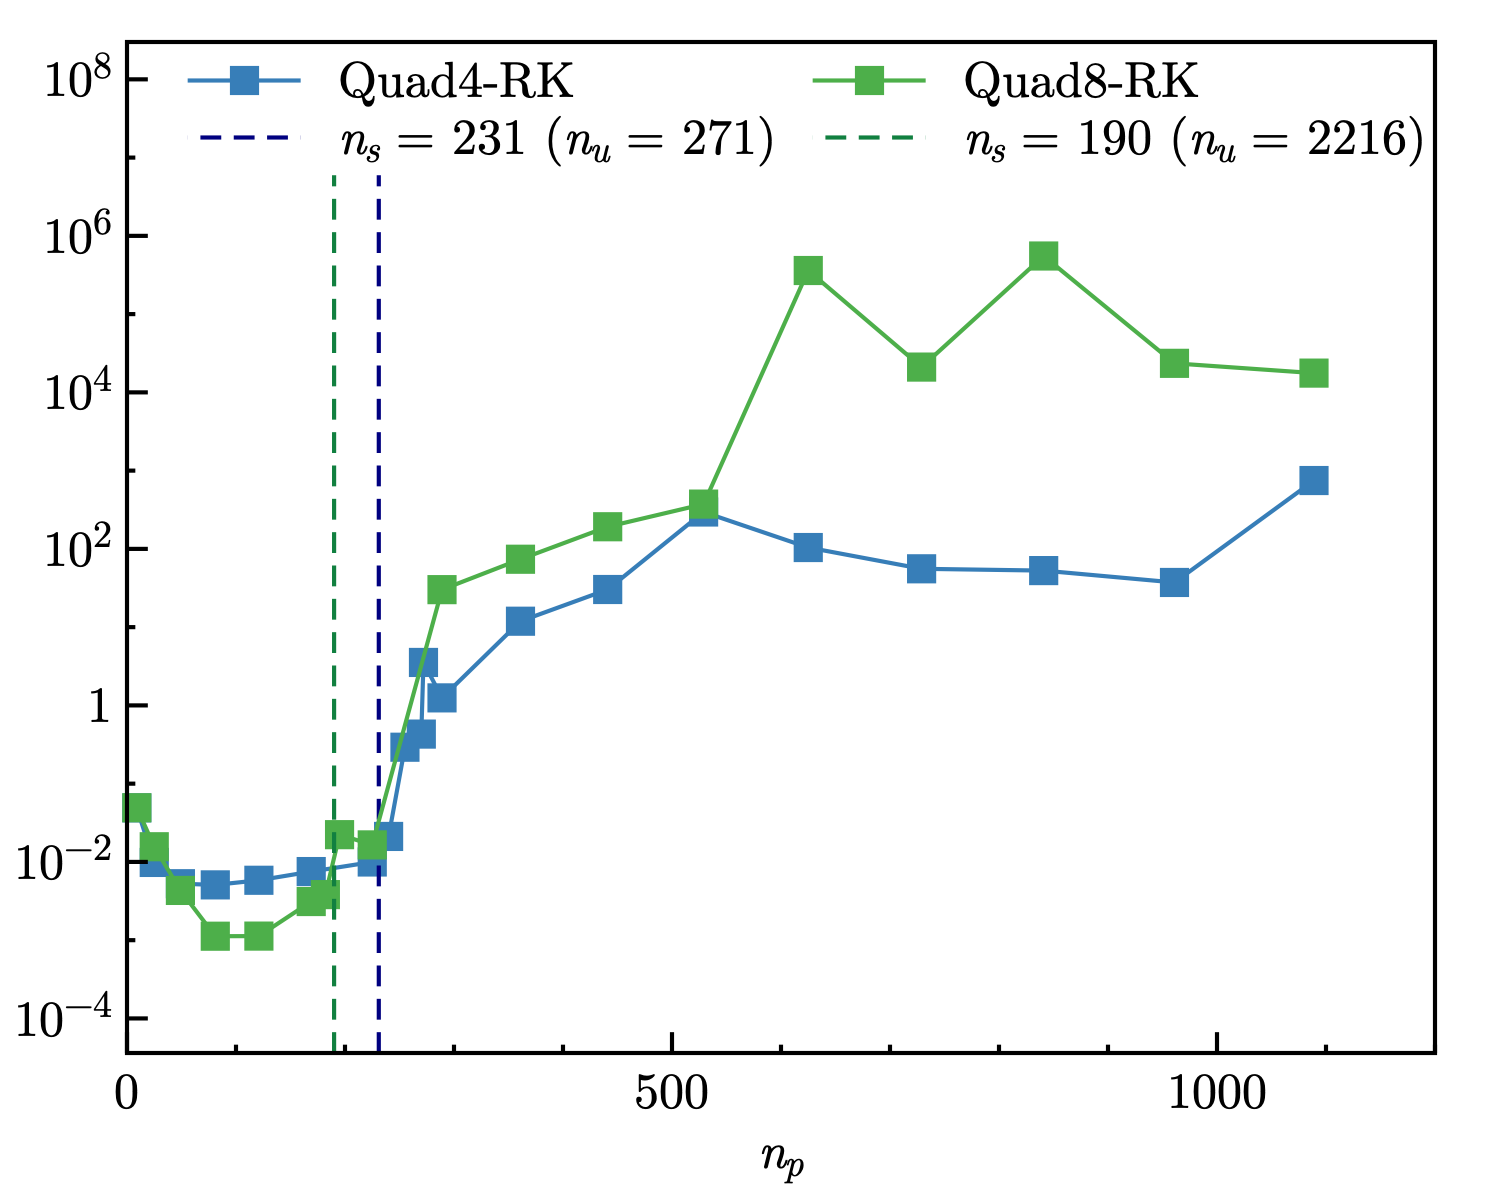
\includegraphics[width=0.48\textwidth]{png/plate_with_hole_quad_L2_p_8.png}} }\\
\DIFaddFL{\raisebox{-0.7\height}{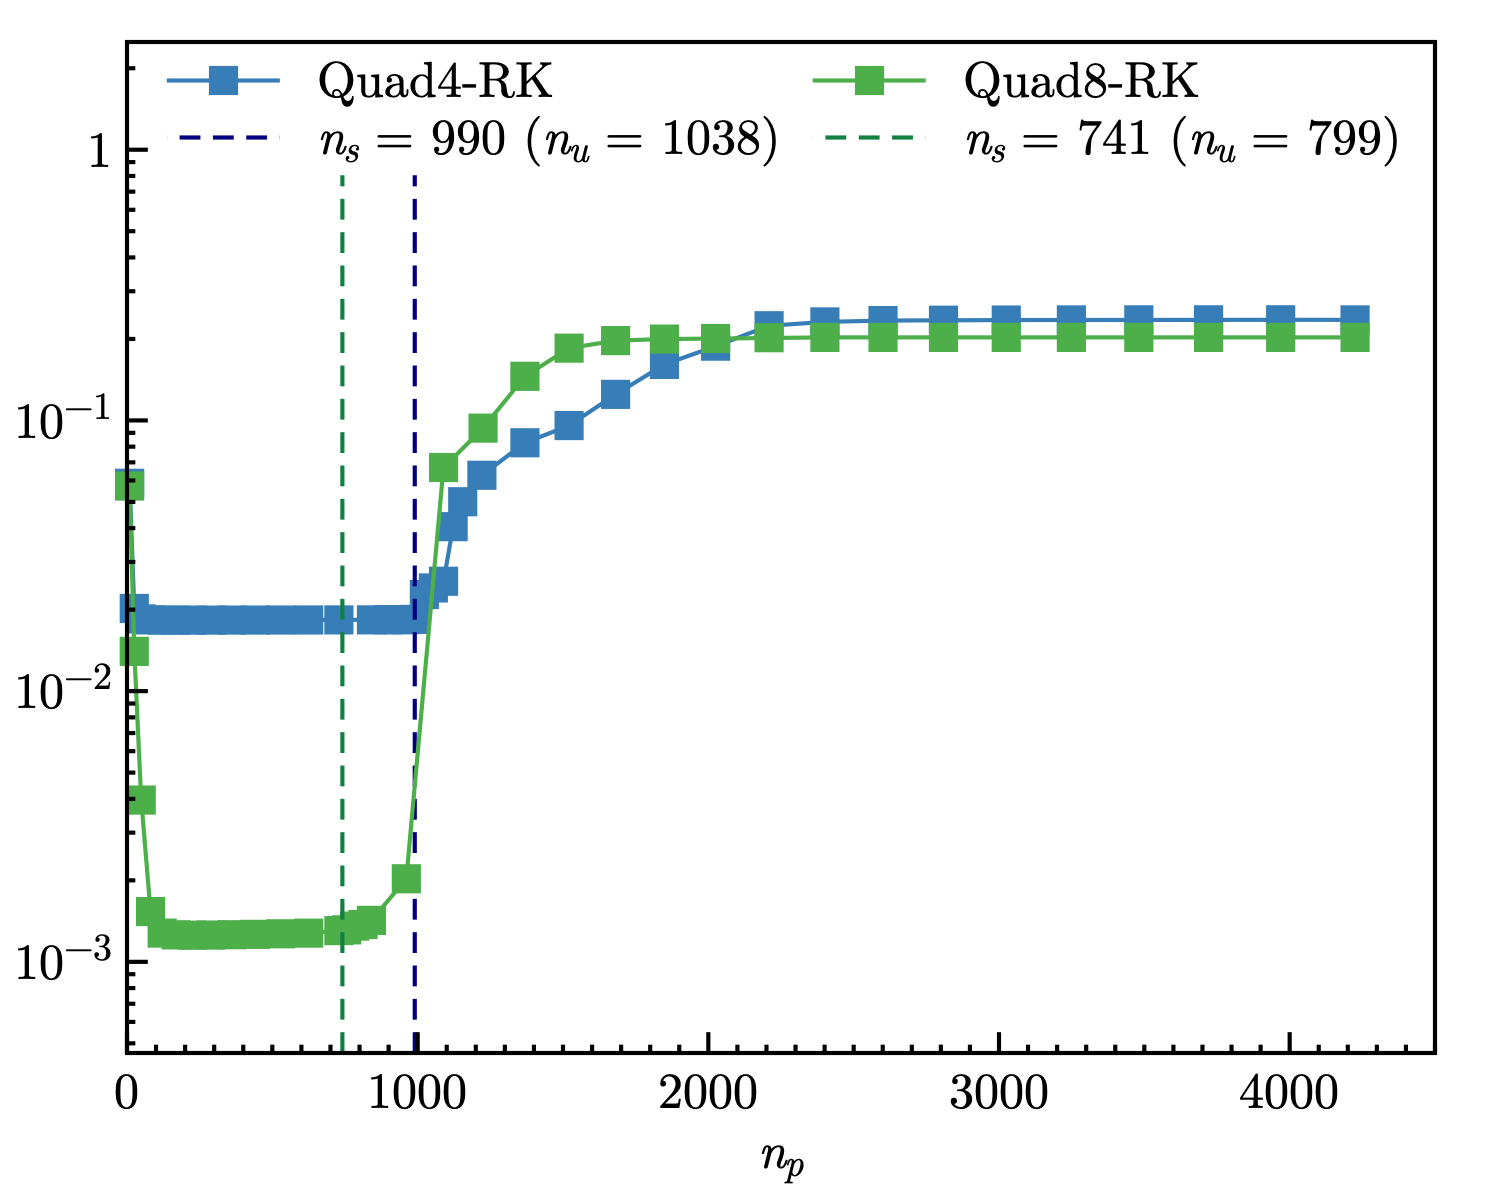
\includegraphics[width=0.48\textwidth]{png/plate_with_hole_quad_Hdev_16.png}}
}& \DIFaddFL{\raisebox{-0.7\height}{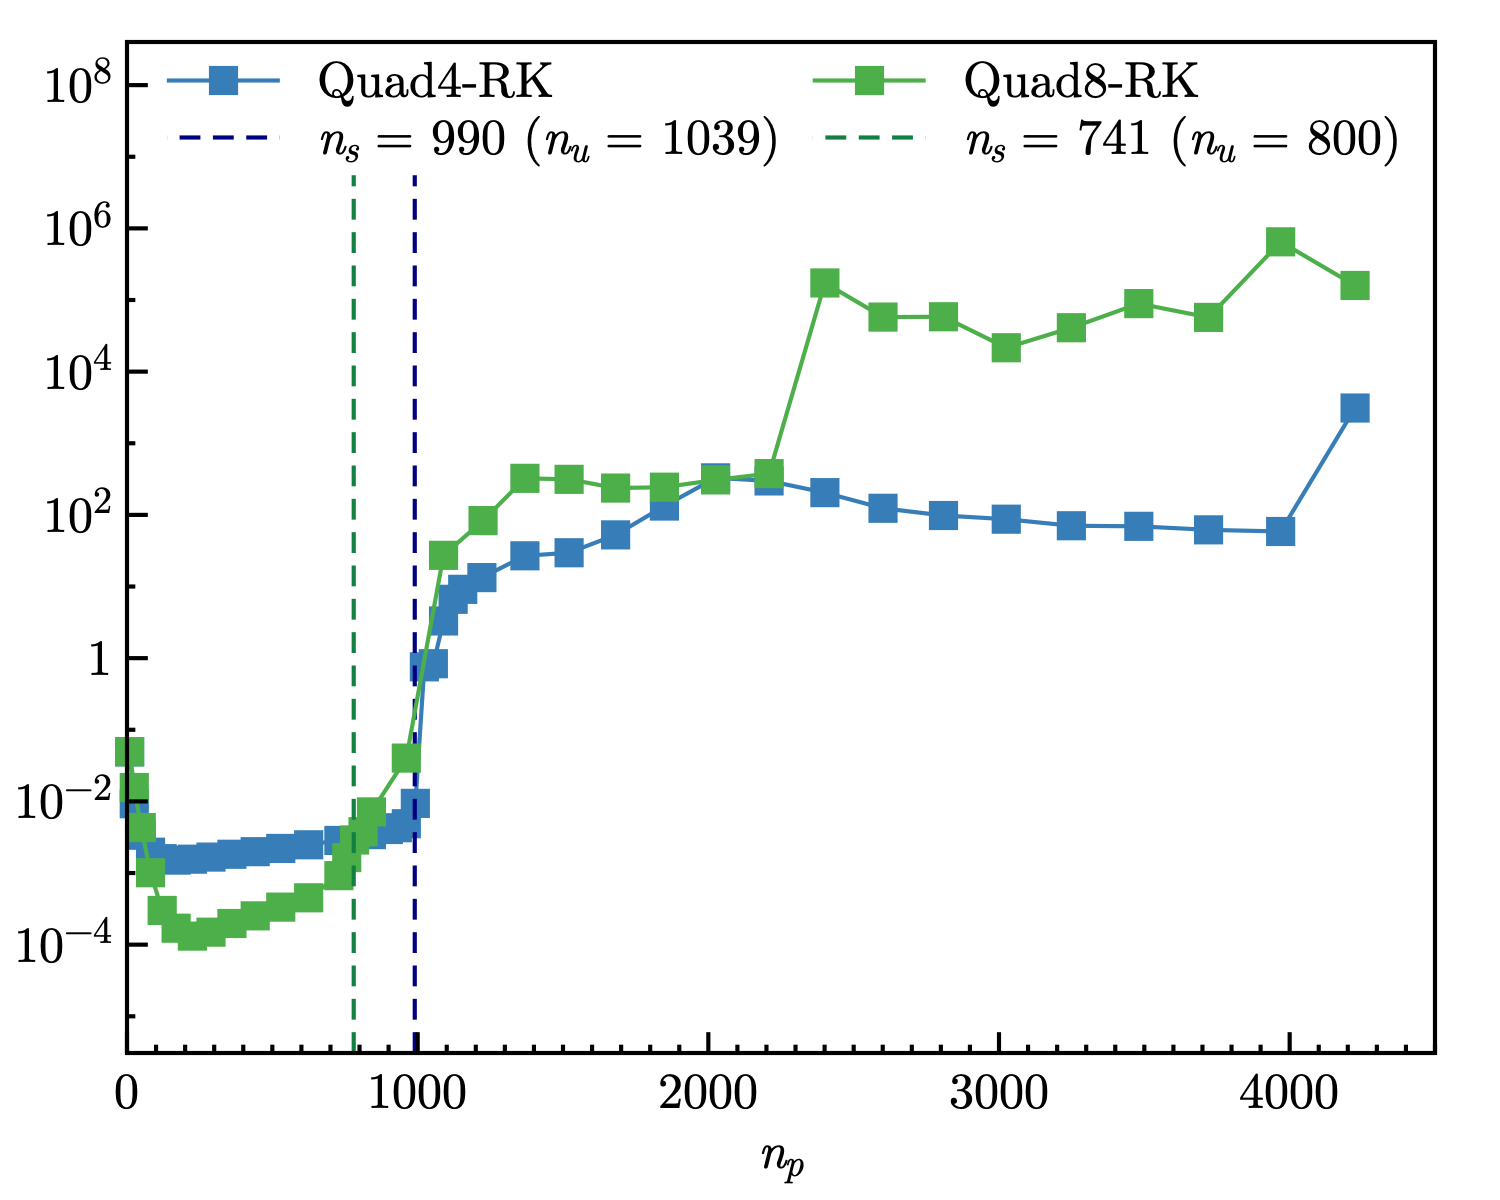
\includegraphics[width=0.48\textwidth]{png/plate_with_hole_quad_L2_p_16.png}} }\\
\DIFaddFL{\raisebox{-0.7\height}{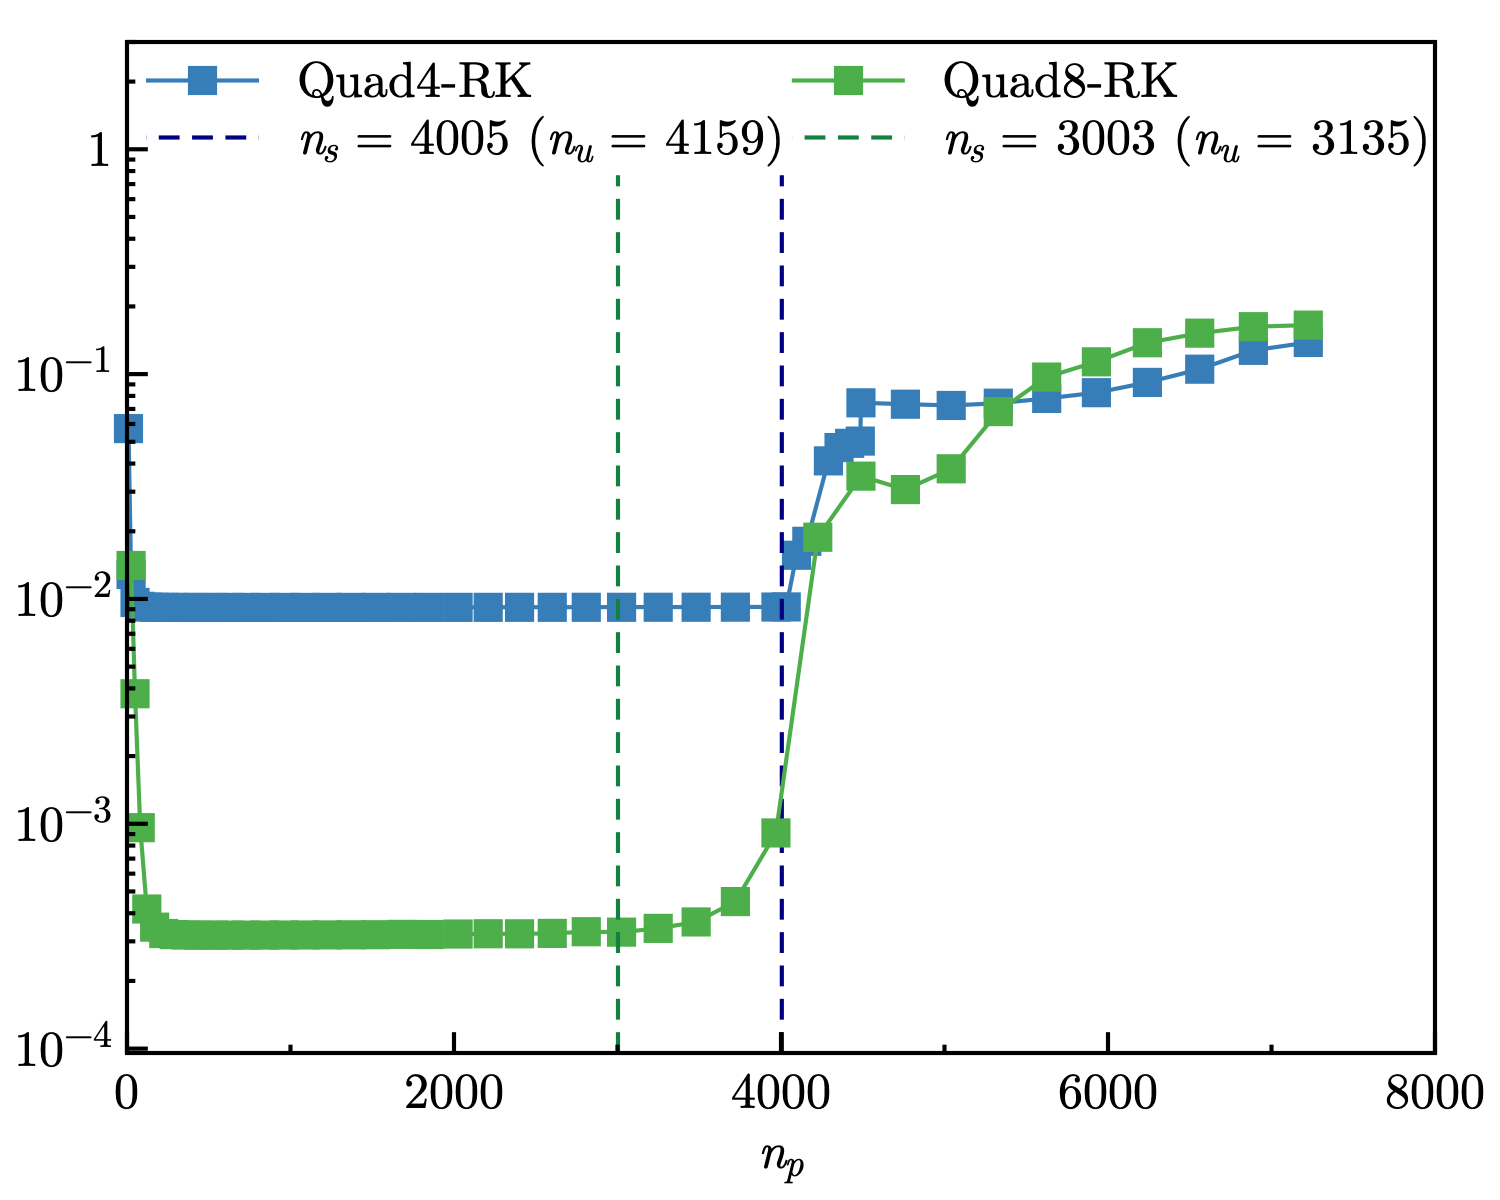
\includegraphics[width=0.48\textwidth]{png/plate_with_hole_quad_Hdev_32.png}}
}& \DIFaddFL{\raisebox{-0.7\height}{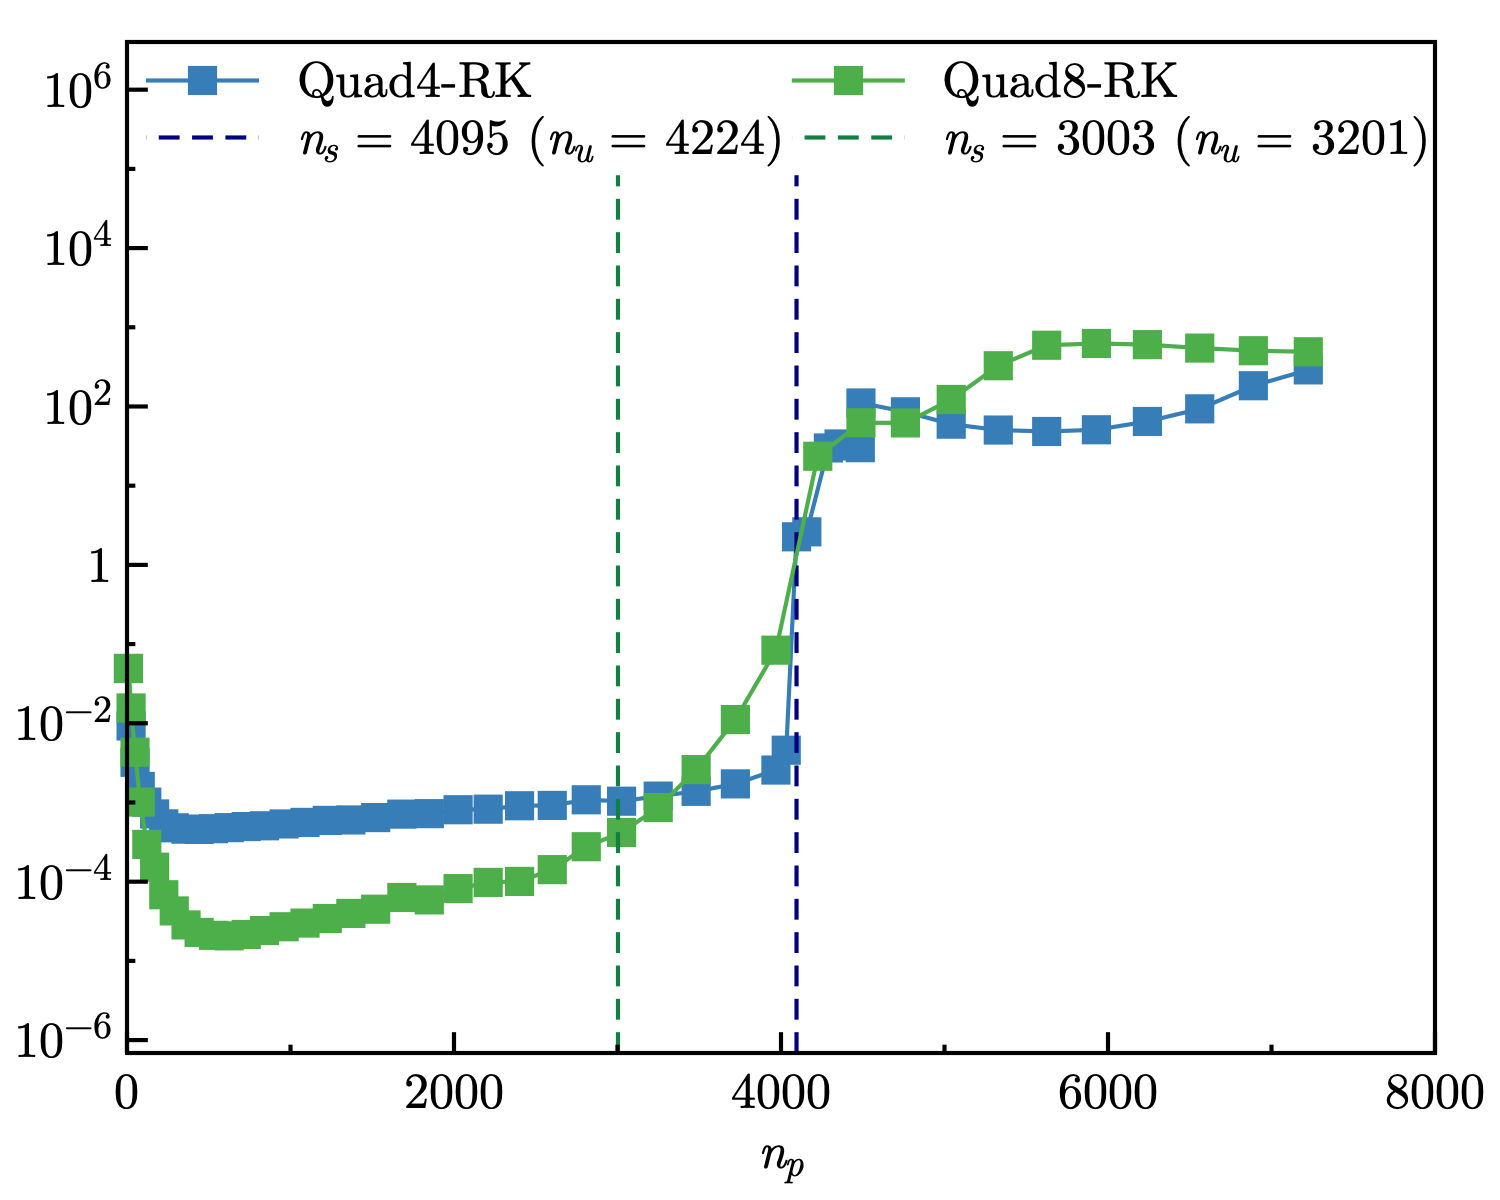
\includegraphics[width=0.48\textwidth]{png/plate_with_hole_quad_L2_p_32.png}} }\\
\end{tabular}
\caption{\DIFaddFL{Strain and pressure errors vs. $n_p$ for plate with hole problem with quadrilateral elements}}\label{fg:plate_with_hole_quad_ns}
\end{figure}

\DIFaddend The corresponding error convergence  \DIFaddbegin \DIFadd{studies are presented in Figures \ref{fg:plate_with_hole_convergence}, \ref{fg:plate_with_hole_convergence_quad}, the }\DIFaddend results show that only Tri3--RK with $r=2$ shows a comparable  \DIFaddbegin \DIFadd{strain error }\DIFaddend with the optimal one with $r=r_{opt}$ \DIFaddbegin \DIFadd{in strain error}\DIFaddend . The other formulations with the traditional constraint ratio show lower accuracy and error convergence rates.

 \DIFaddbegin \begin{figure}[!htp]
\DIFaddendFL \centering
\begin{subcaptiongroup}
\centering
\parbox[b]{0.49\textwidth}{
    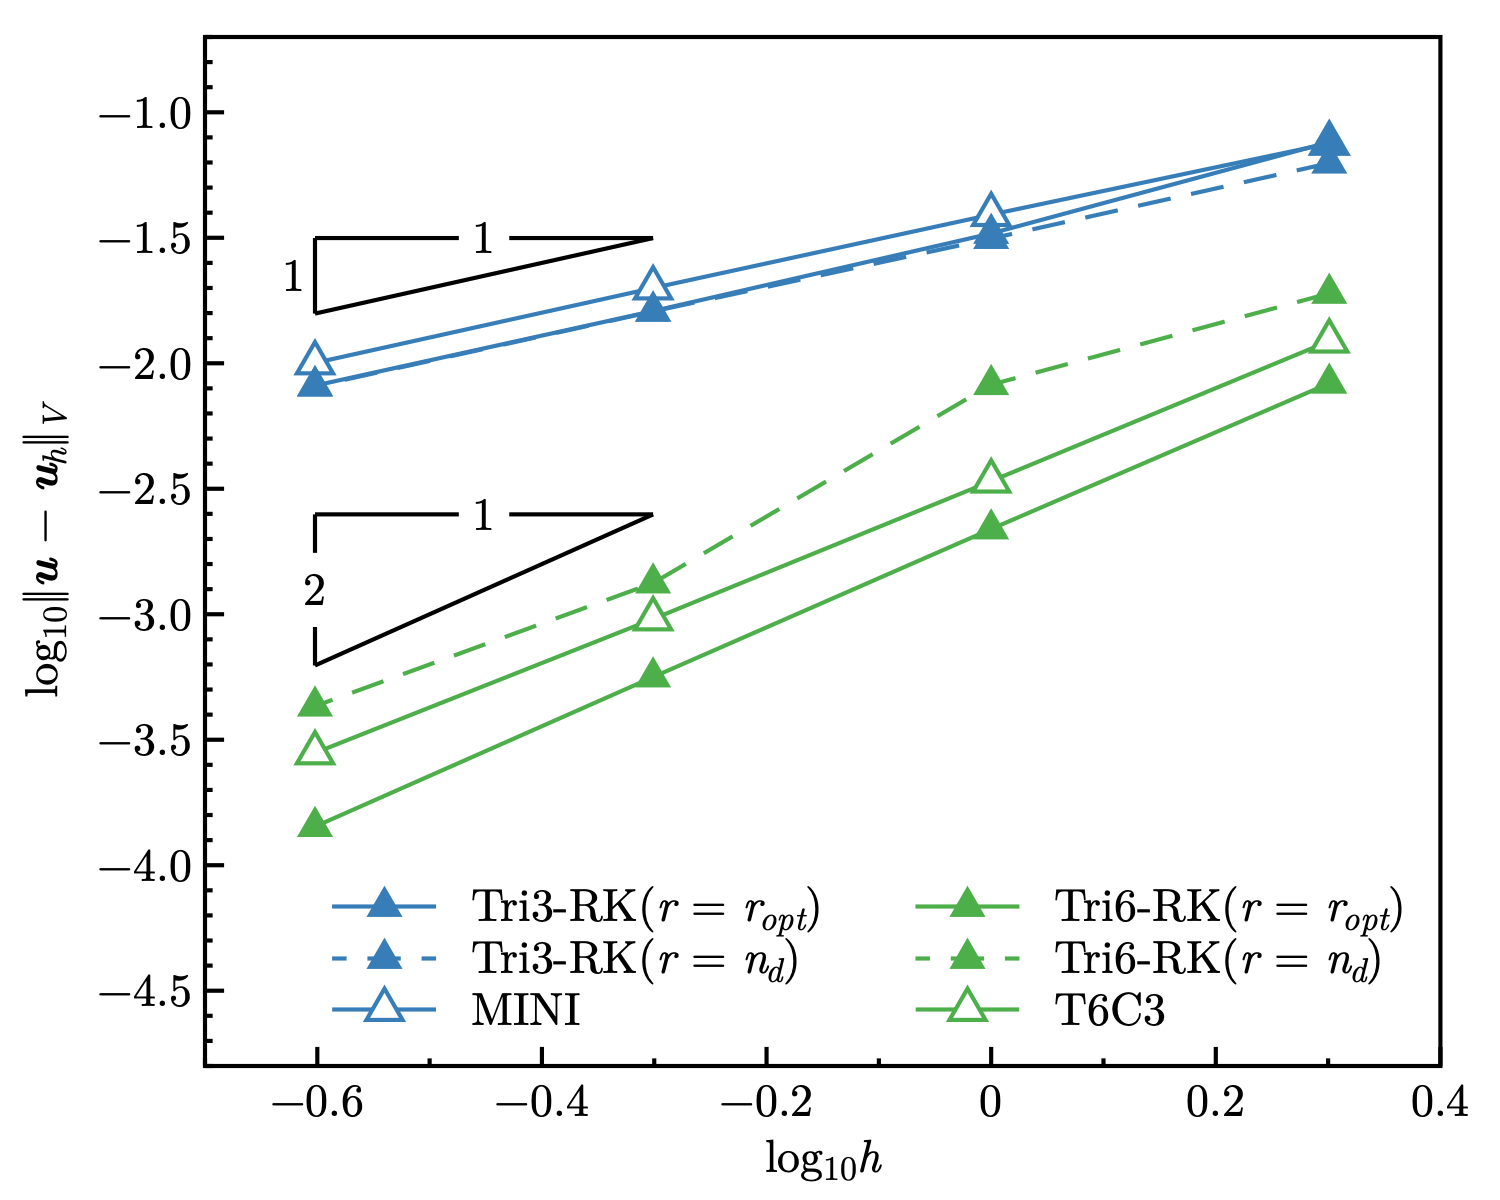
\includegraphics[width=0.49\textwidth]{png/plate_with_hole_Hdev_r1.png}
    \caption{\DIFaddFL{Strain error}}\label{fg:plate_with_hole_convergence_strain}
}
\parbox[b]{0.49\textwidth}{
    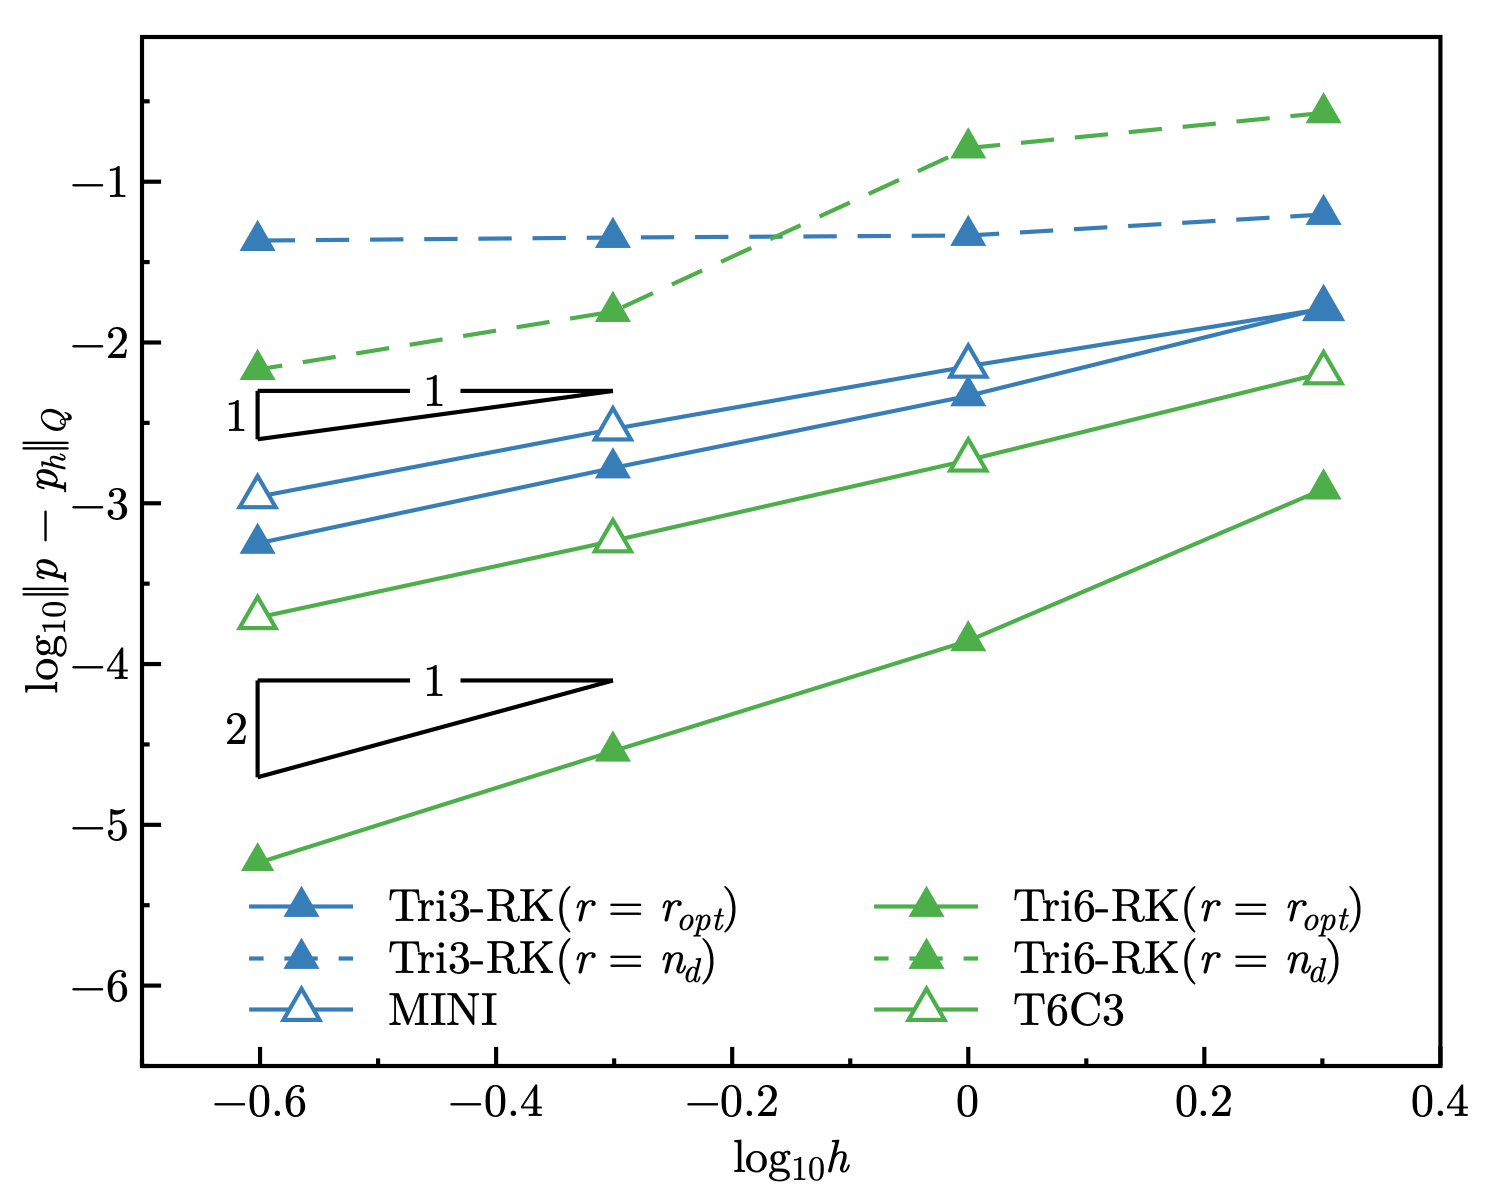
\includegraphics[width=0.49\textwidth]{png/plate_with_hole_L2_p_r1.png}
    \caption{\DIFaddFL{Pressure error}}\label{fg:plate_with_hole_convergence_pressure}
}
\end{subcaptiongroup}
\caption{Error convergence study for plate with hole problem \DIFaddFL{with triangular elements}}\label{fg:plate_with_hole_convergence}
\end{figure}

\begin{figure}[!htp]
\centering
\begin{subcaptiongroup}
\centering
\parbox[b]{0.49\textwidth}{
    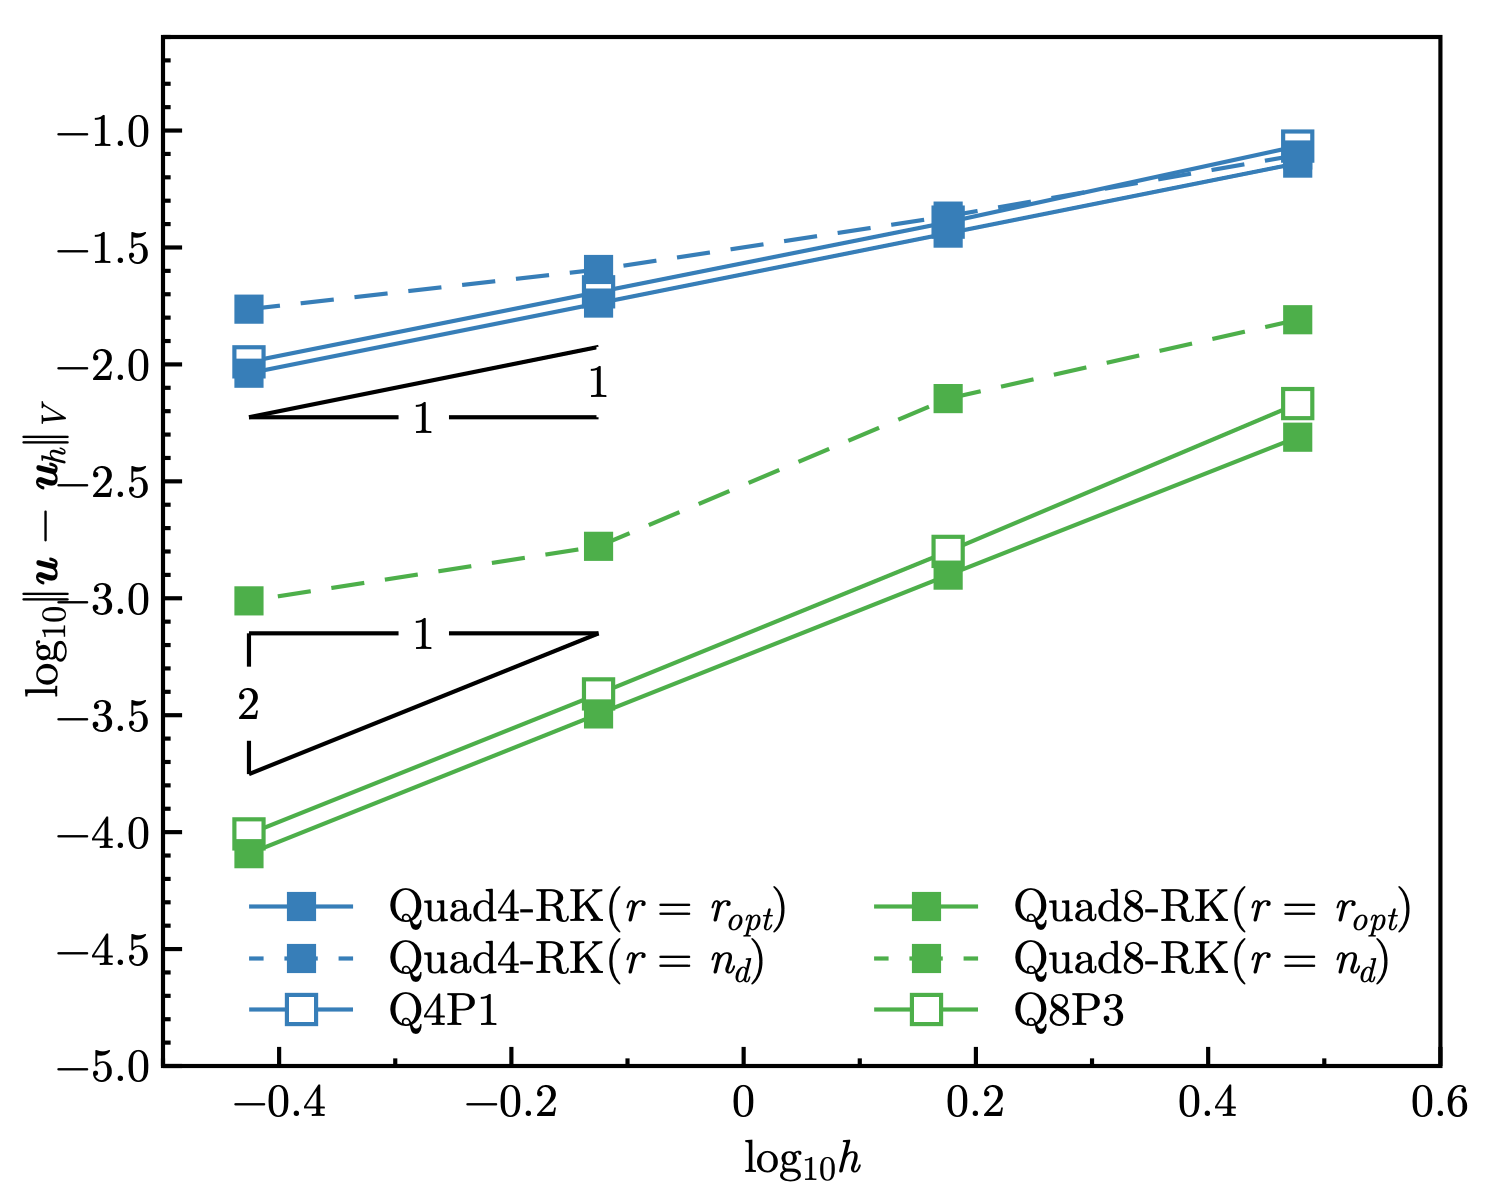
\includegraphics[width=0.49\textwidth]{png/plate_with_hole_quad_Hdev.png}
    \caption{\DIFaddFL{Strain error}}\label{fg:plate_with_hole_convergence_strain_quad}
}
\parbox[b]{0.49\textwidth}{
    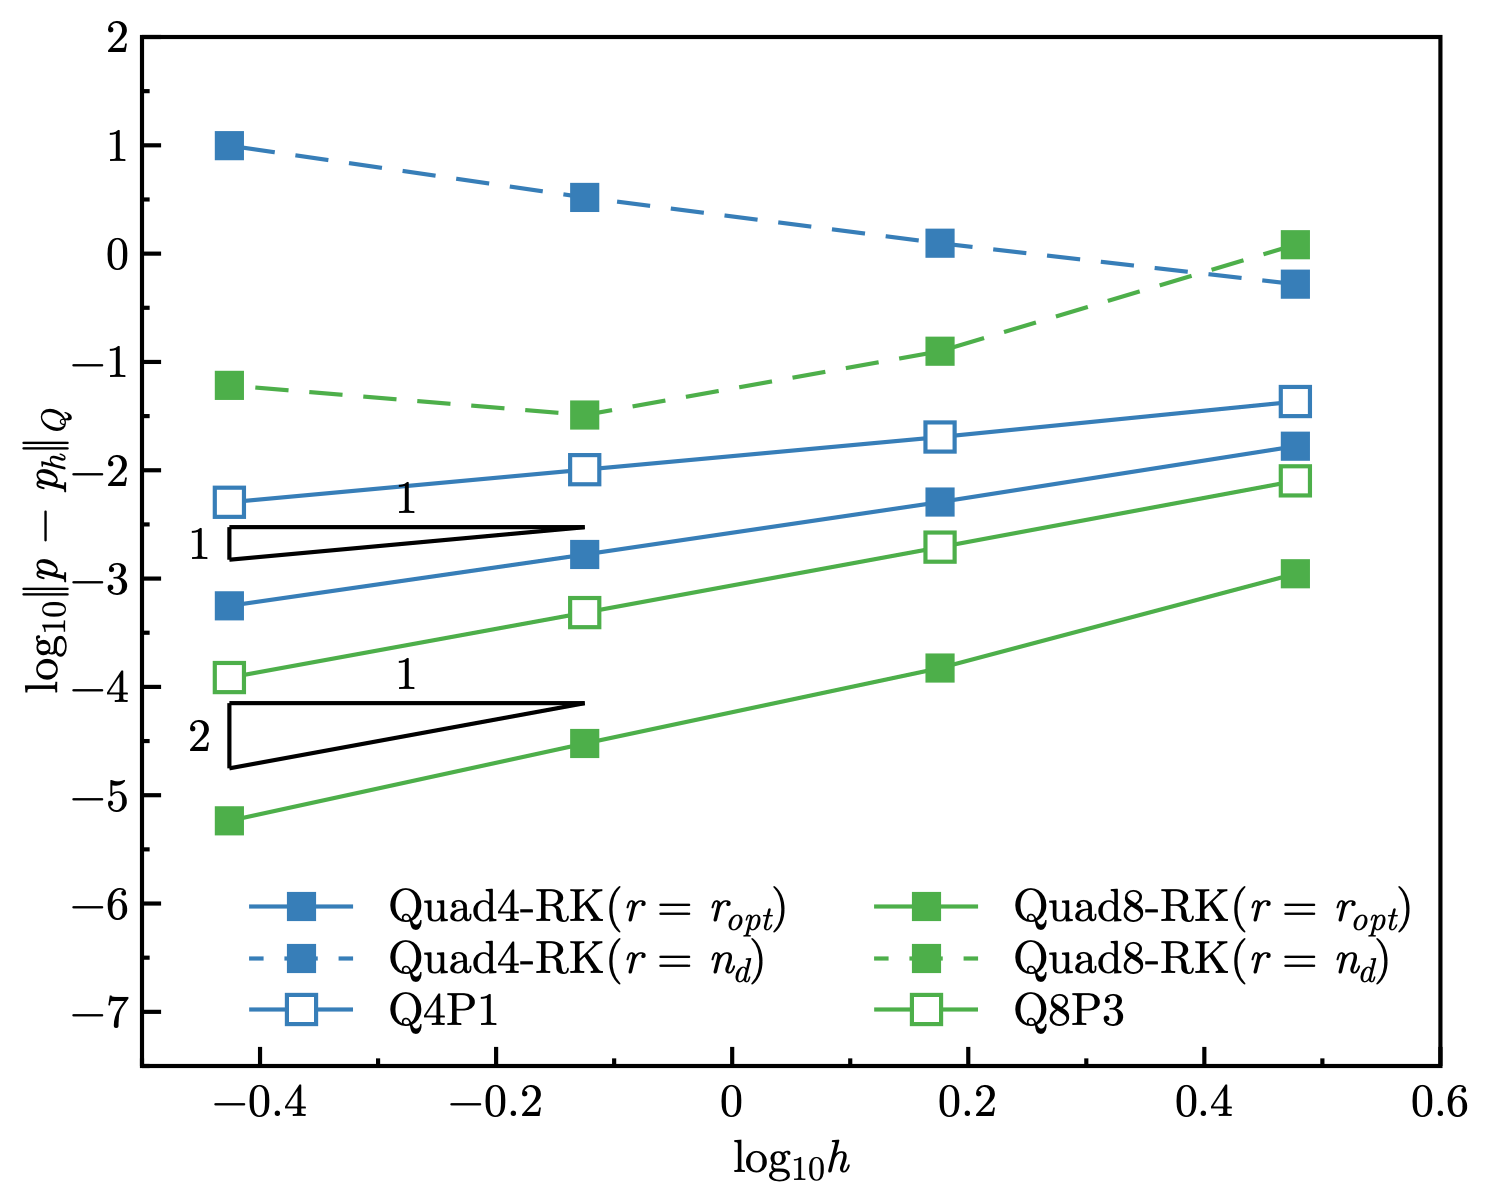
\includegraphics[width=0.49\textwidth]{png/plate_with_hole_quad_L2_p.png}
    \caption{\DIFaddFL{Pressure error}}\label{fg:plate_with_hole_convergence_pressure_quad}
}
\end{subcaptiongroup}
\caption{\DIFaddFL{Error convergence study for plate with hole problem with quadrilateral elements}}\label{fg:plate_with_hole_convergence_quad}
\end{figure}

\DIFadd{Furthermore, the influence of the integration scheme for this problem is investigated.
As shown in Tables \ref{tab_gauss_1} and \ref{tab_gauss_2}, the integration order $n_o$ is varied from 1 to 5 for triangular elements and from 1 to 11 for quadrilateral elements.
The results show that the proposed mixed formulations are not sensitive to the integration order.
Using the traditional lower-order Gauss integration scheme can sufficiently obtain accurate results.
This is consistent with the previous analysis in Section \ref{subsec:rk_approximation}.
}

\begin{table}[!htp]
\centering
\caption{\DIFaddFL{Error comparison with different triangular integration schemes for plate with hole problem}}
\label{tab_gauss_1}
\begin{tabular}{ccccccc}
\toprule
\multirow{2}{*}{$n_o$} &  \DIFaddbeginFL \multirow{2}{*}{$n_g$ for $\Omega$} & \multirow{2}{*}{$n_g$ for $\Gamma$} & \multicolumn{2}{c}{\DIFaddFL{Tri3-RK}} & \multicolumn{2}{c}{\DIFaddFL{Tri6-RK}} \DIFaddendFL \\
 \DIFaddbeginFL \DIFaddFL{\shortstack{} }\DIFaddendFL &  \DIFaddbeginFL \DIFaddFL{\shortstack{} }& \DIFaddFL{\shortstack{} }& \DIFaddFL{$\Vert \boldsymbol u-\boldsymbol u_h \Vert_V$ }& \DIFaddFL{$\Vert p-p_h \Vert_Q$ }& \DIFaddFL{$\Vert \boldsymbol u-\boldsymbol u_h \Vert_V$ }& \DIFaddFL{$\Vert p-p_h \Vert_Q$ }\DIFaddendFL \\
\midrule \DIFaddbeginFL 
\DIFaddFL{1 }\DIFaddendFL &  \DIFaddbeginFL \DIFaddFL{1 }& \DIFaddFL{1 }& \DIFaddFL{3.11E-2 }& \DIFaddFL{3.53E-3 }& \DIFaddFL{8.53E17 }& \DIFaddFL{1.31E4 }\DIFaddendFL \\
 \DIFaddbeginFL \DIFaddFL{2 }\DIFaddendFL &  \DIFaddbeginFL \DIFaddFL{3 }& \DIFaddFL{2 }& \DIFaddFL{3.11E-2 }& \DIFaddFL{3.67E-3 }& \DIFaddFL{8.33E-3 }& \DIFaddFL{1.20E-3 }\DIFaddendFL \\
 \DIFaddbeginFL \DIFaddFL{3 }\DIFaddendFL &  \DIFaddbeginFL \DIFaddFL{4 }& \DIFaddFL{2 }& \DIFaddFL{3.11E-2 }& \DIFaddFL{3.67E-3 }& \DIFaddFL{8.32E-3 }& \DIFaddFL{1.20E-3 }\DIFaddendFL \\
\DIFaddbeginFL \DIFaddFL{4 }& \DIFaddFL{6 }& \DIFaddFL{3 }& \DIFaddFL{3.11E-2 }& \DIFaddFL{3.68E-3 }& \DIFaddFL{8.32E-3 }& \DIFaddFL{1.22E-3 }\\
\DIFaddFL{5 }& \DIFaddFL{7 }& \DIFaddFL{3 }& \DIFaddFL{3.11E-2 }& \DIFaddFL{3.68E-3 }& \DIFaddFL{8.32E-3 }& \DIFaddFL{1.22E-3 }\\
\multicolumn{7}{l}{\footnotesize{$n_o$: Integration order\quad $n_g$: Number of integration points}} \\
\bottomrule
\DIFaddendFL \end{tabular}
 \DIFaddbeginFL \end{table}
\DIFaddend 

 \DIFaddbegin \begin{table}[!htp]
\DIFaddendFL \centering
 \caption{\DIFaddbeginFL \DIFaddFL{Error comparison with different quadrilateral integration schemes for plate with hole problem}\DIFaddendFL}
 \DIFaddbeginFL \label{tab_gauss_2}
\begin{tabular}{ccccccc}
\toprule
\multirow{2}{*}{$n_o$} & \multirow{2}{*}{$n_g$ for $\Omega$} & \multirow{2}{*}{$n_g$ for $\Gamma$} & \multicolumn{2}{c}{\DIFaddFL{Quad4-RK}} & \multicolumn{2}{c}{\DIFaddFL{Quad8-RK}} \\
\DIFaddFL{\shortstack{} }& \DIFaddFL{\shortstack{} }& \DIFaddFL{\shortstack{} }& \DIFaddFL{$\Vert \boldsymbol u-\boldsymbol u_h \Vert_V$ }& \DIFaddFL{$\Vert p-p_h \Vert_Q$ }& \DIFaddFL{$\Vert \boldsymbol u-\boldsymbol u_h \Vert_V$ }& \DIFaddFL{$\Vert p-p_h \Vert_Q$ }\\
\midrule
\DIFaddFL{1 }& \DIFaddFL{3 }& \DIFaddFL{1 }& \DIFaddFL{3.64E-2 }& \DIFaddFL{5.01E-3 }& \DIFaddFL{9.53E13 }& \DIFaddFL{8.15E-1 }\\
\DIFaddFL{3 }& \DIFaddFL{$2\times2$ }& \DIFaddFL{2 }& \DIFaddFL{3.64E-2 }& \DIFaddFL{5.09E-3 }& \DIFaddFL{4.33E-2 }& \DIFaddFL{8.84E-3 }\\
\DIFaddFL{5 }& \DIFaddFL{$3\times3$ }& \DIFaddFL{3 }& \DIFaddFL{3.62E-2 }& \DIFaddFL{3.71E-3 }& \DIFaddFL{1.27E-3 }& \DIFaddFL{4.42E-5 }\\
\DIFaddFL{7 }& \DIFaddFL{$4\times4$ }& \DIFaddFL{4 }& \DIFaddFL{3.62E-2 }& \DIFaddFL{3.70E-3 }& \DIFaddFL{1.26E-3 }& \DIFaddFL{1.49E-4 }\\
\DIFaddFL{9 }& \DIFaddFL{$5\times5$ }& \DIFaddFL{5 }& \DIFaddFL{3.62E-2 }& \DIFaddFL{3.70E-3 }& \DIFaddFL{1.26E-3 }& \DIFaddFL{1.50E-4 }\\
\DIFaddFL{11 }& \DIFaddFL{$6\times6$ }& \DIFaddFL{6 }& \DIFaddFL{3.62E-2 }& \DIFaddFL{3.70E-3 }& \DIFaddFL{1.26E-3 }& \DIFaddFL{1.50E-4 }\\
\multicolumn{7}{l}{\footnotesize{$n_o$: Integration Order\quad $n_g$: Number of integration points}} \\
\bottomrule
\end{tabular}
\end{table}
 \DIFaddend